\documentclass[aps,prb,twocolumn,superscriptaddress,footinbib,amsmath,amssymb,floatfix]{revtex4}
%\documentclass[aps,prb,onecolumn,preprint,superscriptaddress,footinbib,amsmath,amssymb,floatfix]{revtex4}
\usepackage[dvips]{epsfig}
\usepackage{graphicx}
\usepackage{ifthen}
\usepackage{dcolumn}% Align table columns on decimal point
\usepackage{bm}% bold math
\usepackage{multirow}
\usepackage{booktabs}
\usepackage{bm}% bold math
\usepackage{amsbsy}
\usepackage{amsmath}
\usepackage{amssymb}
\usepackage{subfigure}
%\usepackage{wrapfig}

%Definition of new commands
\newcommand{\f}[2]{\ensuremath{\frac{\displaystyle{#1}}{\displaystyle{#2}}}}
\newcommand{\lr}[1]{\langle{#1}\rangle}
\newcommand{\colv}[2] {\left(\begin{array}{c} #1 \\ #2 \end{array}\right)}
\renewcommand{\thefootnote}{\fnsymbol{footnote}}
\newcommand{\be} {\begin{eqnarray}}
\newcommand{\ee} {\end{eqnarray}}
%--------------------------------------------------------------------------
%EQ COMMANDS
%--------------------------------------------------------------------------
\newcommand{\two}{\mspace{-2.0mu}}
\newcommand{\four}{\mspace{-4.0mu}}
\newcommand{\plus}{\mspace{-4.5mu}+\mspace{-3.5mu}}
\newcommand{\minus}{\mspace{-4.5mu}-\mspace{-3.5mu}}
\newcommand{\pp}{'\mspace{-2.0mu}'}
\newcommand{\xlb}[4]{#1\ifthenelse{\equal{#2}{0}}{}{_{\alpha #2}}
\mspace{-2.0mu}\genfrac{(}{)}{0pt}{1}{\ifthenelse{\equal{#3}{0}}{0}{l #3}} 
{\ifthenelse{\equal{#4}{0}}{0}{b #4}}}

\newcommand{\xkv}[4]{#1\mspace{-5.0mu}\left(\mspace{-8.0mu}
\begin{smallmatrix}#2\four{}\four{}\mspace{-8.0mu}&\pmb{\kappa}#3\\&\nu 
#4\end{smallmatrix}\mspace{-5.0mu}\right)}

\newcommand{\evect}[6]{#1\mspace{-4.0mu}\left(\mspace{-8.0mu}
\begin{smallmatrix}#2\mspace{-8.0mu}&\pmb{\kappa} #3 &b #5\\&\nu #4 &
\alpha #6\end{smallmatrix}\mspace{-5.0mu}\right)}

\newcommand{\varmat}[8]{\mspace{-5.0mu}\left(\mspace{-8.0mu}
\begin{smallmatrix}\ifthenelse{\equal{#3}{0}}{\mspace{-8.0mu}&b_{#1}&b_{#2}
\\&\alpha_{#1}&\alpha_{#2}} {\ifthenelse{\equal{#7}{0}}{#1\mspace{-8.0mu}&
\pmb{\kappa}#2#3\mspace{-8.0mu}&\pmb{\kappa}#4#5\mspace{-8.0mu}&\pmb{\kappa}
#6\\&\nu#2&\nu#4&\nu#6} {#1\mspace{-8.0mu}&\pmb{\kappa}#2#3\mspace{-8.0mu}&
\pmb{\kappa}#4#5\mspace{-8.0mu}&\pmb{\kappa}#6#7\mspace{-8.0mu}&\pmb{\kappa}
#8\\&\nu#2&\nu#4&\nu#6&\nu#8}}\end{smallmatrix}\mspace{-5.0mu}\right)}

\newcommand{\EXP}[1]{\exp\mspace{-5.0mu}\left[#1\right]\mspace{-3.0mu}}

\newcommand{\tpp}[2]{\left(\mspace{-2.0mu}\xkv{\omega}{}{}{}#1\xkv{\omega}
{}{'}{'}#2\xkv{\omega}{}{\pp}{\pp}\mspace{-2.0mu}\right)}



%--------------------------------------------------------------------------
\newcommand{\SUM}[2]{\ifthenelse{\equal{#1}{0}}{\sum_{
\alpha_{#2},b_{#2},l_{#2}}^{3,n,N}} {\ifthenelse{\equal{#1}{1}}{\sum_{
\alpha_{#2},b_{#2}}^{3,n}}{\sum_{\pmb{\kappa}#2,\nu#2}^{N,3n}}}}

\newcommand{\SUMprime}[2]{\ifthenelse{\equal{#1}{0}}
{\sum_{\alpha_{#2},b_{#2},l_{#2}}^{3,n,N}} 
{\ifthenelse{\equal{#1}{1}}{\sum_{\alpha_{#2},b_{#2}}^{3,n}}
{\sum_{\pmb{\kappa}^{'}#2,\nu#2}^{N,3n}}}}

\newcommand{\SUMalpha}[2]{\ifthenelse{\equal{#1}{0}}
{\sum_{\alpha_{#2}}^{3}} {\ifthenelse{\equal{#1}{1}}
{\sum_{\alpha_{#2},b_{#2}}^{3,n}}{\sum_{\pmb{\kappa}#2,\nu#2}^{N,3n}}}}
%--------------------------------------------------------------------------
\newcommand{\SUMalphap}[2]{\ifthenelse{\equal{#1}{0}}
{\sum_{\alpha'_{#2}}^{3}} {\ifthenelse{\equal{#1}{1}}
{\sum_{\alpha'_{#2},b'_{#2}}^{3,n}}{\sum_{\pmb{\kappa}#2,\nu#2}^{N,3n}}}}

\newcommand{\SUMb}[2]{\ifthenelse{\equal{#1}{0}}{\sum_{b_{#2}}^{n}}
 {\ifthenelse{\equal{#1}{1}}{\sum_{\alpha_{#2},b_{#2}}^{3,n}}
{\sum_{\pmb{\kappa}#2,\nu#2}^{N,3n}}}}

\newcommand{\SUMbp}[2]{\ifthenelse{\equal{#1}{0}}{\sum_{b'_{#2}}^{n}}
 {\ifthenelse{\equal{#1}{1}}{\sum_{\alpha'_{#2},b'_{#2}}^{3,n}}
{\sum_{\pmb{\kappa}#2,\nu#2}^{N,3n}}}}

\newcommand{\SUMl}[2]{\ifthenelse{\equal{#1}{0}}{\sum_{l_{#2}}^{N}}
 {\ifthenelse{\equal{#1}{1}}{\sum_{\alpha_{#2},b_{#2}}^{3,n}}
{\sum_{\pmb{\kappa}#2,\nu#2}^{N,3n}}}}

\newcommand{\SUMlp}[2]{\ifthenelse{\equal{#1}{0}}{\sum_{l'_{#2}}^{N}}
 {\ifthenelse{\equal{#1}{1}}{\sum_{\alpha'_{#2},b'_{#2}}^{3,n}}
{\sum_{\pmb{\kappa}#2,\nu#2}^{N,3n}}}}

\newcommand{\abcdt}[5]{\mspace{-4.0mu}\left(\mspace{-8.0mu}
\begin{smallmatrix}&\ifthenelse{\equal{#1}{}}{a}{#1}&\ifthenelse
{\equal{#3}{}}{c}{#3}\\&\ifthenelse{\equal{#2}{}}{b}{#2}&\ifthenelse
{\equal{#4}{}}{d}{#4}\end{smallmatrix}\mspace{-2.0mu};\ifthenelse
{\equal{#5}{}}{t}{#5}\right)}

\newcommand{\abcd}[4]{\mspace{-4.0mu}\left(\mspace{-8.0mu}
\begin{smallmatrix}&\ifthenelse{\equal{#1}{}}{a}{#1}&\ifthenelse
{\equal{#3}{}}{c}{#3}\\&\ifthenelse{\equal{#2}{}}{b}{#2}&\ifthenelse
{\equal{#4}{}}{d}{#4}\end{smallmatrix}\mspace{-3.0mu}\right)}

\newcommand{\abt}[3]{\mspace{-4.0mu}\left(\mspace{-8.0mu}\begin
{smallmatrix}&\ifthenelse{\equal{#1}{}}{a}{#1} \\&\ifthenelse{
\equal{#2}{}}{b}{#2}\end{smallmatrix}\mspace{-2.0mu};
\ifthenelse{\equal{#3}{}}{t}{#3}\right)}

\newcommand{\ab}[2]{\mspace{-4.0mu}\left(\mspace{-8.0mu}
\begin{smallmatrix}&\ifthenelse{\equal{#1}{}}{a}{#1} \\&\ifthenelse
{\equal{#2}{}}{b}{#2}\end{smallmatrix}\mspace{-3.0mu}\right)}

\newcommand{\kvbat}{\mspace{-4.0mu}\left(\mspace{-8.0mu}
\begin{smallmatrix} &\pmb{\kappa} &b \\ &\nu &\alpha\end{smallmatrix}
\mspace{-2.0mu};t\right)}
%--------------------------------------------------------------------------


\newcommand{\kgvba}{\mspace{-4.0mu}\left(\mspace{-8.0mu}
\begin{smallmatrix} &\pmb{\kappa}=\pmb{0} &b \\ &\nu 
&\alpha\end{smallmatrix}\mspace{-3.0mu}\right)}

\newcommand{\kgv}{\mspace{-4.0mu}\left(\mspace{-8.0mu}
\begin{smallmatrix}&\pmb{\kappa}=\mathbf{0} \\&\nu\end{smallmatrix}
\mspace{-3.0mu}\right)}

%--------------------------------------------------------------------------

\newcommand{\kvbatp}{\mspace{-4.0mu}\left(\mspace{-8.0mu}
\begin{smallmatrix} &\pmb{\kappa} &b' \\ &\nu &\alpha'\end{smallmatrix}
\mspace{-2.0mu};t\right)}

\newcommand{\kvbaw}{\mspace{-4.0mu}\left(\mspace{-8.0mu}
\begin{smallmatrix} &\pmb{\kappa} &b \\ &\nu &\alpha\end{smallmatrix}
\mspace{-2.0mu};\omega\right)}

\newcommand{\kvbawp}{\mspace{-4.0mu}\left(\mspace{-8.0mu}
\begin{smallmatrix} &\pmb{\kappa} &b' \\ &\nu &\alpha'\end{smallmatrix}
\mspace{-2.0mu};\omega\right)}

\newcommand{\kvba}{\mspace{-4.0mu}\left(\mspace{-8.0mu}
\begin{smallmatrix} &\pmb{\kappa} &b \\ &\nu &\alpha\end{smallmatrix}
\mspace{-3.0mu}\right)}

\newcommand{\kvbap}{\mspace{-4.0mu}\left(\mspace{-8.0mu}
\begin{smallmatrix} &\pmb{\kappa} &b' \\ &\nu &\alpha'\end{smallmatrix}
\mspace{-3.0mu}\right)}
%--------------------------------------------------------------------------
\newcommand{\kpvba}{\mspace{-4.0mu}\left(\mspace{-8.0mu}
\begin{smallmatrix} &\pmb{\kappa}^{'} &b \\ &\nu &\alpha\end{smallmatrix}
\mspace{-3.0mu}\right)}

\newcommand{\kva}{\mspace{-4.0mu}\left(\mspace{-8.0mu}
\begin{smallmatrix} &\pmb{\kappa} \\ &\nu &\alpha\end{smallmatrix}
\mspace{-3.0mu}\right)}

\newcommand{\kvap}{\mspace{-4.0mu}\left(\mspace{-8.0mu}
\begin{smallmatrix} &\pmb{\kappa} \\ &\nu &\alpha'\end{smallmatrix}
\mspace{-3.0mu}\right)}

\newcommand{\kvb}{\mspace{-4.0mu}\left(\mspace{-8.0mu}
\begin{smallmatrix} &\pmb{\kappa} &b \\ &\nu \end{smallmatrix}
\mspace{-3.0mu}\right)}

\newcommand{\kvbp}{\mspace{-4.0mu}\left(\mspace{-8.0mu}
\begin{smallmatrix} &\pmb{\kappa} &b' \\ &\nu \end{smallmatrix}
\mspace{-3.0mu}\right)}

\newcommand{\kvt}{\mspace{-4.0mu}\left(\mspace{-8.0mu}
\begin{smallmatrix}&\pmb{\kappa} \\&\nu\end{smallmatrix}
\mspace{-2.0mu};t\right)}

\newcommand{\kgvt}{\mspace{-4.0mu}\left(\mspace{-8.0mu}
\begin{smallmatrix}&\pmb{\kappa=0} \\&\nu\end{smallmatrix}
\mspace{-2.0mu};t\right)}

\newcommand{\kpvt}{\mspace{-4.0mu}\left(\mspace{-8.0mu}
\begin{smallmatrix}&\pmb{\kappa}^{'} \\&\nu\end{smallmatrix}
\mspace{-2.0mu};t\right)}

\newcommand{\kvw}{\mspace{-4.0mu}\left(\mspace{-8.0mu}
\begin{smallmatrix}&\pmb{\kappa} \\&\nu\end{smallmatrix}
\mspace{-2.0mu};\omega\right)}

\newcommand{\kv}{\mspace{-4.0mu}\left(\mspace{-8.0mu}
\begin{smallmatrix}&\pmb{\kappa} \\&\nu\end{smallmatrix}
\mspace{-3.0mu}\right)}

\newcommand{\kw}{\mspace{-4.0mu}\left(\mspace{-8.0mu}
\begin{smallmatrix}&\pmb{\kappa} \\&\omega\end{smallmatrix}
\mspace{-3.0mu}\right)}

\newcommand{\knw}{\mspace{-4.0mu}\left(\mspace{-8.0mu}
\begin{smallmatrix}&\pmb{\kappa} \\&\omega\end{smallmatrix}
\mspace{-3.0mu}\right)}

\newcommand{\kpvp}{\mspace{-4.0mu}\left(\mspace{-8.0mu}
\begin{smallmatrix}&\pmb{\kappa'} \\&\nu'\end{smallmatrix}
\mspace{-3.0mu}\right)}
%--------------------------------------------------------------------------
\newcommand{\lbt}{\mspace{-4.0mu}\left(\mspace{-8.0mu}
\begin{smallmatrix}&l \\&b\end{smallmatrix}\mspace{-2.0mu};t\right)}

\newcommand{\lbtp}{\mspace{-4.0mu}\left(\mspace{-8.0mu}
\begin{smallmatrix}&l' \\&b'\end{smallmatrix}\mspace{-2.0mu};t\right)}

\newcommand{\lt}{\mspace{-4.0mu}\left(\mspace{-8.0mu}
\begin{smallmatrix}&l\end{smallmatrix}\mspace{-2.0mu};t\right)}

\newcommand{\ltp}{\mspace{-4.0mu}\left(\mspace{-8.0mu}
\begin{smallmatrix}&l'\end{smallmatrix}\mspace{-2.0mu};t\right)}

\newcommand{\lb}{\mspace{-4.0mu}\left(\mspace{-8.0mu}
\begin{smallmatrix}&l \\&b\end{smallmatrix}\mspace{-3.0mu}\right)}

\newcommand{\lbp}{\mspace{-4.0mu}\left(\mspace{-8.0mu}
\begin{smallmatrix}&l' \\&b'\end{smallmatrix}\mspace{-3.0mu}\right)}
%--------------------------------------------------------------------------
%COMMANDS
%--------------------------------------------------------------------------
\begin{document}
%--------------------------------------------------------------------------
\title{Thermal Conductivity Accumulation in Amorphous Materials}
%--------------------------------------------------------------------------
\author{Jason M. Larkin}
\author{Alan J. H. McGaughey}
\affiliation{Department of Mechanical Engineering\\
Carnegie Mellon University\\Pittsburgh, PA 15213}
%\email[]{mcgaughey@cmu.edu}
%--------------------------------------------------------------------------
\date{\today}
%--------------------------------------------------------------------------
\begin{abstract}

By definition, phonons are non-localized propagating vibrations that 
transport energy over distances much larger than the atomic spacing. For 
amorphous solids, with the 
exception 
of very long-wavelength (low-frequency) modes, the vibrational modes are 
non-propagating. 
Recently, 
experimental measurements of the thermal conductivity of amorphous 
materials demonstrate that 
propagating (phonon-like) modes with large mean free paths 
contribute significantly to thermal transport in amorphous 
materials.\cite{regner_broadband_2013,sultan_heat_2013} 
Using broadband frequency domain thermal-reflectance, 
Regner et al. measured how the thermal conductivity of a-SiO$_2$ and 
a-Si thin films change with the penetration depth associated with the 
heating laser pulse.\cite{regner_broadband_2013} 
Regner et al. argue that their measurements probe the mean free 
paths of propagating vibrational modes to measure the 
thermal conductivity accumulation function.    
Using lattice dynamics calculations and molecular dynamics simulations 
on 
realistic models of a-SiO$_2$ and a-Si, we predict and 
characterize the contributions from propagating and non-propagating 
vibrations 
to thermal conductivity. The vibrational mean free paths 
and (for the first time) the thermal 
conductivity accumulation functions are predicted for a-SiO$_2$ and a-Si 
and compared with experimental results of 
Regner et al. and varying thin film measurements. 
For a-SiO$_2$, the propagating modes are found to contribute 
negligibly for both bulk and thin films. We demonstrate the scaling 
of the low-frequency propagating mode diffusivities using 
(to our knowledge) the largest model of bulk a-Si.   
For a-Si, the propagating modes contribute significantly to thermal 
transport. We consider two scalings of the propagating mode 
diffusivities to compare with the results of Regner et al. and thin 
film measurements and find 
good qualitative agreement for both. Further 
experiments are suggested based on our predictions and the comparisons. 
\end{abstract}
%--------------------------------------------------------------------------
\maketitle
%--------------------------------------------------------------------------
%\clearpage
\section{\label{S:Introduction}Introduction}
%--------------------------------------------------------------------------

% Amorphous silicon (a-Si) and nanocrystalline silicon have applications 
% in high-efficiency solar cells.(cite) 
% Films and substrates made of a-SiO$_2$ and a-Si have wide application in 
% semiconductor and optoelectronic devices.
% (cite) Understanding the thermal transport in these amorphous systems 
% is critical to improving their performance. 
% Thermal transport at scales comparable to phonon wave-
% lengths and mean free paths (MFPs) is presently a topic of
% considerable interest for both crystalline and amorphous materials.
% \cite{cahill_nanoscale_2003,
% yu_reduction_2010,hochbaum_enhanced_2008,pernot_precise_2010}
% Recently, nanostructured materials
% such as nanowires, superlattices, and composites with
% strongly reduced thermal conductivities due to phonon
% scattering at interfaces and boundaries.
% \cite{hochbaum_enhanced_2008,pernot_precise_2010,
% boukai_silicon_2008,poudel_high-thermoelectric_2008} 

The Allen and Feldman (AF) theory for disordered solids   
classifies vibrational modes in a disordered system as 
propagating (propagons, i.e. phonon-like), 
non-propagating (diffusons), and 
localized (locons).\cite{allen_thermal_1993,allen_diffusons_1999} 
Several experimental measurements and estimates based on experiments 
demonstrate that propagating modes contribute significantly 
for amorphous silicon nitride\cite{sultan_heat_2013} and
amorphous silicon (a-Si),\cite{cahill_thermal_1994,liu_high_2009,
yang_anomalously_2010} 
but not 
a-SiO$_2$.\cite{love_estimate_1990,lee_heat_1997,baldi_thermal_2008} 
Using broadband frequency domain thermal-reflectance, 
Regner et al. measured how the thermal conductivity of a-SiO$_2$ and 
a-Si thin films change with the penetration depth associated with the 
heating laser pulse.\cite{regner_broadband_2013} 
For a-SiO$_2$, the thermal conductivity of a 1000 nm 
film did not vary for penetration depths between 57 and 960 nm, 
suggesting that any propagating modes that contribute to thermal 
conductivity have MFPs below 57 nm. For a-Si, they find the 
thermal conductivities of thin films between 500 and 2000 nm 
vary by about 
40$\%$ for penetration depths between 44 and 968 nm, suggesting 
that propagating modes with MFPs of 100 to 1000 nm contribute 
significantly to thermal conductivity.\cite{regner_broadband_2013}  
Following the suggestion of Koh and Cahill, they interpret the 
measured value at a given penetration depth to be representative 
of the phonons with MFP less than that value, allowing for the 
construction of the so-called thermal conductivity accumulation 
function.\cite{dames_thermal_2005,minnich_thermal_2011,
yang_mean_2013}

To understand the results of Regner et al. requires knowledge of 
the MFPs of the 
propagating modes and the contribution from non-propagating modes. 
Experimentally, inelastic neutron scattering has been
used to measure phonon lifetimes (MFPs) in materials,
but this technique is more suited for single crystal samples.
\cite{christianson_phonon_2008} 
An x-ray diffraction and thermoreflectance technique
can measure ballistic transport in some structures, but is 
not well-suited for amorphous thin films.
\cite{highland_ballistic-phonon_2007} 
Traditionally, empirical expressions and
simple models have been the only means
to estimate MFPs in amorphous materials.
\cite{zeller_thermal_1971,graebner_phonon_1986,
freeman_thermal_1986,cahill_lattice_1988,cahill_heat_1989} 
Because of this, the thermal conductivity accumulation 
function in amorphous materials is still not well understood.
\cite{feldman_thermal_1993,cahill_thermal_1994,
feldman_numerical_1999,liu_high_2009,yang_anomalously_2010,
he_heat_2011,regner_broadband_2013}

Interpreting the measured thermal conductivity accumulation 
functions 
requires an understanding of how the MFPs of the 
low-frequency propagating modes scale with frequency.
\cite{freeman_thermal_1986,graebner_phonon_1986,
love_estimate_1990,feldman_thermal_1993,cahill_thermal_1994,
feldman_numerical_1999,baldi_thermal_2008,liu_high_2009,
yang_anomalously_2010} 
Experimental measurements of the thermal conductivity of
thin films of a-SiO$_2$ and a-Si at varying temperatures 
gives indirect information about the low-frequency propagating 
modes.\cite{freeman_thermal_1986,graebner_phonon_1986,
love_estimate_1990,feldman_thermal_1993,cahill_thermal_1994,
feldman_numerical_1999,zink_thermal_2006,baldi_thermal_2008,
liu_high_2009,yang_anomalously_2010,hondongwa_ultrasonic_2011} 
For a-SiO$_2$, varying temperature 
and film thickness
\cite{graebner_phonon_1986,freeman_thermal_1986,
cahill_lattice_1988,cahill_heat_1989,love_estimate_1990,
lee_heat_1997,yamane_measurement_2002,baldi_thermal_2008} 
measurements all suggest that the propagating modes 
contribute a negligible amount to thermal conductivity. 
However, the behavior of the low-frequency modes 
has only recently been understood by experimental 
measurements.
\cite{masciovecchio_evidence_2006,baldi_thermal_2008,
baldi_sound_2010,baldi_elastic_2011,baldi_emergence_2013} 
For a-Si the low-frequency behavior of the MFPs is less understood.
\cite{feldman_thermal_1993,cahill_thermal_1994,
feldman_numerical_1999,zink_thermal_2006,liu_high_2009,
yang_anomalously_2010,he_heat_2011,hondongwa_ultrasonic_2011} 
Temperature-varying\cite{zink_thermal_2006} 
and film thickness-varying measurements
\cite{pompe_thermal_1988,cahill_thermal_1989,hasselman_thermal_1989,
kuo_thermal_1992,feldman_thermal_1993,cahill_thermal_1994,
wada_thermal_1996,feldman_numerical_1999,
moon_thermal_2002,zink_thermal_2006,zink_excess_2006,liu_high_2009,
yang_anomalously_2010}
suggest multiple different behavior of the low-frequency 
scaling of the mean free paths of vibrational modes in a-Si. 

The objective of this work is to investigate the propagating 
and non-propagating contributions to thermal conductivity of 
a-SiO2 and a-Si 
by predicting the MFPs and thermal conductivity 
accumulation functions for realistic models to 
compare with recent measurements by Regner et al.
\cite{regner_broadband_2013} and experimental measurements 
for varying film thicknesses at 300 K.
\cite{freeman_thermal_1986,graebner_phonon_1986,
cahill_lattice_1988,cahill_thermal_1989,
love_estimate_1990,cahill_thermal_1994,lee_heat_1997,
yamane_measurement_2002,baldi_thermal_2008,
liu_high_2009,yang_anomalously_2010} The paper is organized as follows. 
Using the Green-Kubo method and 
molecular dynamics (MD) simulations of large, realistic atomistic models 
of bulk a-SiO$_2$ and a-Si (including, to our 
knowledge, the largest MD simulation for a model of a-Si
\cite{barkema_high-quality_2000,he_heat_2011}), 
we predict the total thermal conductivity in Section \ref{S:Bulk}. 
Using MD simulations and lattice dynamics calculations, 
we predict the propagating and non-propagating mode 
diffusivities using a bottom-up approach 
based on the mode-by-mode properties in Section \ref{S:Diffusivities} and 
the the total thermal conductivity in Section \ref{S:Bulk} to compare with 
the GK method predictions. 
From the bottom-up approach, the spectrum of vibrational MFPs and 
the thermal conductivity accumulation functions 
are predicted for the first time 
for a-SiO$_2$ and a-Si in Section \ref{S:Accumulation} and 
compared with the measurements of  
Regner et al.\cite{regner_broadband_2013} and experiments on 
thin films.\cite{freeman_thermal_1986,graebner_phonon_1986,
cahill_lattice_1988,cahill_thermal_1989,
love_estimate_1990,cahill_thermal_1994,lee_heat_1997,
yamane_measurement_2002,baldi_thermal_2008,
liu_high_2009,yang_anomalously_2010} 
Further experimentation 
is suggested based on the predictions from our models, previous 
experiments,
\cite{freeman_thermal_1986,graebner_phonon_1986,
cahill_lattice_1988,cahill_thermal_1989,
love_estimate_1990,cahill_thermal_1994,lee_heat_1997,
yamane_measurement_2002,baldi_thermal_2008,
liu_high_2009,yang_anomalously_2010}
and emerging broadband thermoreflectance techniques.
\cite{koh_frequency_2007,minnich_thermal_2011,regner_broadband_2013,
yang_mean_2013}

% (NOT HERE)
% While predictions for the contributions to the total 
% vibrational thermal conductivity $k_{vib}$ from 
% propagating ($k_{pr}$) and non-propagating ($k_{AF}$) have 
% been made for a-SiO$_2$ and a-Si,(cite) no thermal conductivity 
% accumulation functions have been predicted to compare with Regner.
% (cite) 
% Using lattice dynamics calculations and molecular dynamics simulations 
% of large-scale ($~4000$ atom models), 
% we predict the inputs to Eq. \eqref{EQ:kvib} in Sections \ref{S:DOS}, 
% \ref{S:Structure}, \ref{S:Diffusivities}, and the bulk thermal 
% conductivity 
% $k_{vib}$ and its contributions $k_{pr}$ and $k_{AF}$ in Section 
% \ref{S:Bulk} 
% Using very large-scale (up to $800,000$ atoms) 
% MD simulations, we predict the thermal 
% thermal conductivity $k_{vib}$ of bulk a-SiO$_2$ and a-Si to compare with 
% the predictions based on the mode-by-mode properties. 
% For the first time, the MFPs of propagating modes in bulk 
% a-SiO$_2$ and a-Si are used with a boundary scattering model 
% to predict the thermal conductivity accumulation, which is 
% compared with experimental thin film measurements and broadband 
% FDTR measurements of a-SiO$_2$ and a-Si in Section \ref{S:Accumulation}.

% w4
% 
% phenomologically suggested
% \cite{zeller_thermal_1971,graebner_phonon_1986} 
% percolation lattice
% \cite{sheng_heat_1991}
% Rayleigh\cite{wischnewski_sound-wave_1998}
% Rayleigh\cite{ganter_rayleigh_2010} 
% numerical study of disordered lattices with varying coordination 
% show Rayleigh type scattering.\cite{wyart_scaling_2010} 
% 
% w2
% 
% model of a-SiO$_2$ shows $\omega^{-2}$\cite{taraskin_propagation_2000}
% 
% \cite{ciliberti_brillouin_2003}
% 
% w4 and w2
% 
% \cite{baldi_thermal_2008,baldi_sound_2010,baldi_emergence_2013} 
% inconclusive evidence\cite{feldman_calculations_2002}
% cross-over shown theoretically
% \cite{schirmacher_thermal_2006,schmid_raman_2008,
% schirmacher_vibrational_2008}
% 
% This perplexing property of glasses
% has been explained heuristically by assuming that phonons
% are scattered so strongly by structural disorder that trans-
% port becomes diffusive, with a frequency regime of small,
% constant thermal diffusivity.
% \cite{kittel_interpretation_1949,sheng_heat_1991,allen_thermal_1993} 
% 
% Fabian and Allen predict w2 dependance for model of a-Si.
% \cite{fabian_theory_1999}
% 
% shows $\tau ~ \omega^{-2}$ for a hard-sphere model.
% \cite{gotze_evolution_2000} 
% shows w2 scaling of the inverse linewdiths from structure factor of model 
% glasses.\cite{shintani_universal_2008}
% shows w2 for long, w2.5 for tran for a model of a-SiO$_2$.
% \cite{horbach_high_2001}
% 
% review paper on aiSO2: models and experimental data for a-SiO$_2$ shows w2 for 
% short wavelength, high frequency modes and scaling near w2.5 at low frequency.
% \cite{ruocco_high-frequency_2001} 
% 
% Using theory based on the random spatial variation of the shear modulus, 
% a transition from w4 to w2 scaling is observed at frequencies much lower
% than the so-called ``Boson peak`` frequency.
% \cite{schirmacher_acoustic_2007}
% 
% experiment from Benassi et al. show a $k^2$ 
% dependance.\cite{benassi_evidence_1996}
% 
% a-Si
% Christie et al. find a best fit of w2.5 for a model of a-Si, although 
% adequate fits to w2 and w4 were shown.\cite{christie_vibrational_2007} 
% 
% The nature of vibrations in amorphous systems in this
% frequency region is not yet fully understood. It is known
% that a force-constant-disordered crystalline lattice gives 
% w4,\cite{schirmacher_harmonic_1998,taraskin_origin_2001} 
% while many positionally disordered materials, including a-Si, 
% give w2, as does a positionally disordered analytical model.
% \cite{martin-mayor_dynamical_2001,ciliberti_brillouin_2003} 
% 
% It may therefore be positional disorder which is responsible 
% for the reduction
% in the exponent from 4 to 2, although the mechanism of
% this reduction remains unclear. Of particular interest is
% the recent experimental work of Masciovecchio et al.,
% \cite{masciovecchio_evidence_2006}
% which suggests that there may be three regimes in vitreous
% silica, with respectively w2 to w4 and back to w2. If this
% behavior is generally true, then these regions could occur
% at different ranges of wavevector for different materials,
% and this could account for different dependences being
% observed between different materials; the w4 dependence in 
% lithium diborate,\cite{ruffle_observation_2003} and for 
% the intermediate value
% of exponent 2.54 found for the transverse polarization
% by Christie et al.\cite{christie_vibrational_2007} and others.
% 
% In conclusion we have shown that in a system without any
% periodic order such as a monatomic liquid, one observes in-
% elastic excitations that can be interpreted as the noncrystal-
% line counterpart of Umklapp peaks.\cite{scopigno_observation_2001} 
% 
% The goal of this work...
% 
% In this work, we consider two ``stiff glass'' amorphous systems:
% Structural relxation phenomena do not dominate the dynamics 
% of the.\cite{gotze_evolution_2000} 
% 
% For modeling the low frequency vibrational modes, two types of 
% scattering mechanisms are considered: (a) phonon-phonon 
% scattering (b) Rayleigh scattering.

% The goal of this work is to predict the MFP of vibrational modes in 
% disordered systems. Simple Lennard-Jones systems will be studied.  A 
% perfect LJ crystal are alloyed with a species of differing mass and 
% amorphous samples are prepared. Thermal transport will be studied to 
% quantify and characterize the ordered and 
% disordered contributions to lattice thermal conductivity. In particular, a 
% more rigorous way to classify vibrational modes in disordered alloys and 
% amorphous samples as phonon-like or diffuson will be investigated. These 
% results will be compared to the phenomenological Einstein and Cahill-Pohl 
% models,\cite{einstein1911,kittel1949,cahill1992}.

% hermal conductivity (k), which relates the heat flux (!
% q)
% and temperature gradient (rT) in a material through the
% Fourier law, !
% q 1⁄4 À krT, results from the cumulative
% contributions of phonons with a broad range of mean free paths
% (MFPs). The spectral MFP distribution is critical in nanostruc-
% tured materials and devices, where size effects selectively scatter
% phonons or create non-Fourier conduction based on individual
% phonon MFPs. Such effects have an impact on heat dissipation in
% nanoelectronics and photonics, as well as the design of
% nanostructured thermoelectric materials with reduced thermal
% conductivity1–9. Because of its ubiquity in electronics, crystalline
% silicon (c-Si) has emerged as the prototypical material of study,
% yet controversy persists on what phonon MFPs dominate thermal
% transport, even in the bulk material. Kinetic theory defines the
% thermal conductivity as k 1⁄4 Cvs LG =3, where C is the volumetric
% heat capacity, vs is the speed of sound and LG is the average
% (or grey) MFP. For c-Si, kinetic theory yields LG 1⁄4 41 nm at a
% temperature (T) of 300 K10. This grey approximation severely
% underestimates the MFPs of the phonons that contribute
% significantly to thermal conductivity because (i) dispersion
% makes vs an overestimate of the average group velocity of
% acoustic phonons and (ii) optical phonons contribute to C but
% negligibly to bulk k (ref. 11). Thermal conductivity measurements
% of thin silicon films indicate that an effective MFP of 300 nm at
% T 1⁄4 300 K is more appropriate12.

% Non-local
% Another type of size effect can occur if
% there is a temperature gradient over length scales compa-
% rable to phonon MFPs. In this case, local thermal equilib-
% rium does not exist and the transport is nondiffusive.
% Transient ballistic transport has been studied using heat-
% pulse techniques at cryogenic temperatures [8].
% \cite{von_gutfeld_heat_1964} 
% A nonlocal
% theory of heat transport was proposed as a modification of
% diffusion theory [9].\cite{mahan_nonlocal_1988} 
% It was also predicted that the heat
% conduction from a nanoparticle is significantly reduced
% from the Fourier law prediction.\cite{chen_particularities_2000}

%--------------------------------------------------------------------------
\section{\label{S:Theory:Thermal}Theoretical Formulation of 
Vibrational Thermal Conductivity}
%--------------------------------------------------------------------------

We calculate the total vibrational thermal conductivity, $k_{vib}$, 
of an amorphous solid from 
\begin{equation}\label{EQ:kvib}
\begin{split}
k_{vib} = k_{pr} + k_{AF},
\end{split}
\end{equation}
where $k_{pr}$ is the contribution from 
propagating (phonon-like) modes\cite{ashcroft_solid_1976,
dove_introduction_1993,ziman_electrons_2001} 
and $k_{AF}$ is the contribution 
from diffusons (i.e., delocalized, non-propagating modes) predicted 
by the AF theory.\cite{feldman_thermal_1993} Mode level 
properties obtained from MD simulations and lattice dynamics 
calculations will be used as inputs. 
The form of Eq. \eqref{EQ:kvib} has been used in 
previous studies of amorphous materials,
\cite{graebner_phonon_1986,freeman_thermal_1986,
love_estimate_1990,feldman_thermal_1993,cahill_thermal_1994,
feldman_numerical_1999,baldi_thermal_2008,
liu_high_2009,yang_anomalously_2010} 
all leading to predictions that while $k_{pr}$ is a negligible 
fraction of $k_{vib}$ for a-SiO$_2$ ($< 10\%$),
\cite{love_estimate_1990,baldi_thermal_2008} 
it is non-negligible 
for a-Si($> 20\%$).
\cite{feldman_thermal_1993,cahill_thermal_1994,
feldman_numerical_1999,liu_high_2009,yang_anomalously_2010,
he_heat_2011}

The propagating contribution is modeled as
\cite{feldman_thermal_1993,feldman_numerical_1999} 
\begin{equation}\label{EQ:kph}
\begin{split}
k_{pr} = \frac{1}{V}\int_{0}^{\omega_{cut}} 
DOS(\omega) C(\omega) D_{pr}(\omega)d\omega,
\end{split}
\end{equation}
where $V$ is the system volume, $\omega$ is the mode 
frequency, $\omega_{cut}$ is the maximum frequency of propagating 
modes,  
$DOS(\omega)$ is the vibrational 
density of states, $C(\omega)$ is the mode specific heat, 
and $D_{pr}(\omega)$ is the mode diffusivity. When using mode 
properties obtained from finite-sized systems, it is more common 
to write Eq. \eqref{EQ:kph} as a summation over the available modes. 
We choose the integral form because the required use of finite-sized 
simulation cells limit the lowest frequency 
modes that can be accessed and an extrapolation 
must be made to the zero frequency limit.
\cite{love_estimate_1990,feldman_thermal_1993,cahill_thermal_1994,
feldman_numerical_1999,baldi_thermal_2008,
liu_high_2009,yang_anomalously_2010}    
Equation \eqref{EQ:kph} is obtained by using the single-mode relaxation
time approximation to solve 
the Boltzmann transport equation for a phonon gas.
\cite{ziman_electrons_2001} In the derivation of Eq. 
\eqref{EQ:kph}, the system is assumed to be isotropic 
(valid for an amorphous material) 
and have a single polarization,\cite{dove_introduction_1993} 
making the mode properties only a function of frequency. The 
choice of single polarization (i.e., an averaging 
of the transverse and longitudinal branches) 
does not significantly change the results predicted in this work  
or that of others.
\cite{feldman_thermal_1993,cahill_thermal_1994,
feldman_numerical_1999,baldi_thermal_2008,liu_high_2009,
yang_anomalously_2010} 
% We write Eq. \eqref{EQ:kph} in terms of the 
% mode diffusivities to align with the diffuson theory,
% \cite{feldman_thermal_1993} which 
% is described later in this Section. 
We will evaluate Eq. \eqref{EQ:kph} under the Debye approximation, 
which assumes isotropic and linear dispersion such that the 
the density of states is
\begin{equation}\label{EQ:DOS_debye}
DOS(\omega) = \frac{3\pi\omega^2}{2v_{s}^3},
\end{equation}
where $v_s$ is an appropriate sound speed.\cite{ashcroft_solid_1976} 


Because MD simulations are classical,\cite{mcquarrie_statistical_2000} 
we take the specific heat to be $k_{\text{B}}$ in the 
harmonic limit, where $k_{\text{B}}$ is the Boltzmann constant. 
This harmonic approximation has been shown to be valid 
for a-Si modeled using the Stillinger-Weber (SW) potential at the temperature 
of interest here (300 K),\cite{feldman_thermal_1993} and is generally 
valid for a range of systems such as 
Lennard-Jones (LJ) argon\cite{mcgaughey_quantitative_2004} 
and carbon nanotubes\cite{larkin_comparison_2012} for temperatures less 
than half the melting temperature. 
Taking the classical limit for the specific heat allows for a direct 
comparison between the MD- and lattice dynamics-based 
predictions. 
The full quantum expression for the specific heat is
\cite{ziman_electrons_2001}
\begin{equation}\label{EQ:Cquantum}
\begin{split}
C(\omega) = k_{\text{B}}\left[\frac{\hbar\omega/2k_{\text{B}}T}
{\text{sinh}(\hbar\omega/2k_{\text{B}}T)}\right]^2.
\end{split}
\end{equation} 
The quantum specific heat is used for the high-frequency 
diffuson modes 
predicted using lattice dynamics to compare our predictions 
for $k_{AF}$ to experimental measurements in Sections 
\ref{S:Bulk} and \ref{S:Accumulation}. 

The diffusivity of the propagating modes is    
\begin{equation}\label{EQ:Dtau}
\begin{split}
D_{pr}(\omega) = \frac{1}{3}v^2_s\tau(\omega),
\end{split}
\end{equation}
where $\tau(\omega)$ is the frequency-dependent mode 
lifetime.\cite{ziman_electrons_2001} An equivalent physical 
picture in terms of a scattering length is
\begin{equation}\label{EQ:DLambda}
\begin{split}
D_{pr}(\omega) = \frac{1}{3}v_s \Lambda(\omega),
\end{split}
\end{equation}
where $\Lambda(\omega)$ is the phonon mean free path (MFP), defined as 
\begin{equation}\label{EQ:Lambda}
\begin{split}
\Lambda(\omega) = v_{s} \tau(\omega).
\end{split}
\end{equation}
The lifetimes will be modeled using 
\begin{equation}\label{EQ:tauw2}
\begin{split}
\tau(\omega) = B \omega^{-n}.
\end{split}
\end{equation}
For amorphous materials, the scaling exponent $n$ 
has been found experimentally and numerically to be 
between two and four,
\cite{vacher_ultrasonic_1981,
feldman_thermal_1993,morath_phonon_1996,benassi_evidence_1996,
feldman_numerical_1999,taraskin_determination_1999,
taraskin_propagation_2000,gotze_evolution_2000,ruocco_relaxation_2000,
ruocco_high-frequency_2001,horbach_high_2001,
matic_sound_2001,
feldman_calculations_2002,ruffle_observation_2003,
masciovecchio_evidence_2006,schirmacher_acoustic_2007,
christie_vibrational_2007,
shintani_universal_2008,xu_energy_2009,
liu_high_2009,ganter_rayleigh_2010,
vitelli_heat_2010,
baldi_sound_2010,yang_anomalously_2010,
wyart_scaling_2010,baldi_elastic_2011,
he_heat_2011,ayrinhac_subterahertz_2011,
baldi_emergence_2013}
where a value of two corresponds to 
Umklapp scattering\cite{callaway_model_1959} and a value of four 
corresponds to 
Rayleigh scattering from point defects.\cite{klemens_scattering_1955}
Combined with the form of the $DOS(\omega)$ 
[Eq. \eqref{EQ:DOS_debye}], choosing $n\le2$ ensures that the 
thermal conductivity evaluated from Eq. \eqref{EQ:kph} is finite. 
Choosing $n>2$ causes the thermal conductivity to diverge,   
which can be fixed using additional anharmonic
\cite{feldman_thermal_1993,feldman_numerical_1999} 
or boundary scattering terms.
\cite{cahill_thermal_1994,liu_high_2009,yang_anomalously_2010}

The AF diffuson contribution to thermal conductivity is
\cite{feldman_thermal_1993,feldman_numerical_1999}
\begin{equation}\label{EQ:kAF}
\begin{split}
k_{AF} = \frac{1}{V}\sum_{i,\omega_i>\omega_{cut}} 
C(\omega_i) D_{AF}(\omega_i), 
\end{split}
\end{equation}
where $\omega_i$ is the frequency of the $i$th diffuson mode, 
$C(\omega_i)$ is the diffuson specific heat, and $D_{AF}(\omega_i)$ 
is the diffuson diffusivity. Equation \eqref{EQ:kAF} is written as a 
sum because there are enough high-frequency diffusons in the 
finite-size systems studied here to ensure a converged 
value.\cite{feldman_thermal_1993,feldman_numerical_1999} 
% Written as an integral, Eq. \eqref{EQL:kAF} has the same form as 
% Eq. \ref{EQ:kph}, which can be derived starting 
% with the Kubo theory
% \cite{flicker_lattice_1973,allen_thermal_1993,alam_lattice_2005,
% baldi_thermal_2008,yang_anomalously_2010}  
% and taking the limit 
% of zero phonon self-energy.\cite{baldi_thermal_2008} 
The AF diffusivities are calculated from\cite{allen_thermal_1993} 
\begin{equation}\label{EQ:DAF}
\begin{split}
D_{AF}(\omega_i) = \frac{\pi V^2}{\hbar^2\omega^2_i}\sum_{j\neq i}
|S_{ij}|^2 \delta(\omega_i - \omega_j),
\end{split}
\end{equation}
where $\hbar$ the Planck constant and $\delta$ is the Dirac delta 
function. The heat current operator $S_{ij}$ measures the thermal 
coupling 
between vibrational modes $i$ and $j$ based on their frequencies and 
spatial overlap of eigenvectors, 
can be calculated from harmonic lattice dynamics theory.
\cite{allen_thermal_1993,feldman_thermal_1993,feldman_numerical_1999} 
For Eq. \eqref{EQ:DAF}, $S_{ij}$ is directionally averaged because 
the amorphous materials studied in this work are isotropic. 

%%--------------------------------------------------------------------------
%\subsection{\label{S:Limits}Thermal Conductivity and Diffusivity Limits}
%%--------------------------------------------------------------------------

% To interpret the non-propagating contribution $k_{AF}$, it is useful 
% to consider a high-scatter (HS) limit for the mode diffusivity,
% \begin{equation}\label{EQ:D_HS}
% D_{HS} = \frac{1}{3} v_s a,
% \end{equation}
% where it is assumed that all vibrational modes travel with the sound speed  
% $v_s$ and scatter over a distance of the lattice constant $a$.
% \cite{cahill_lattice_1988}  
% Equation \eqref{EQ:D_HS} leads to a high-scatter (HS) limit of 
% thermal conductivity in the classical limit given by
% \cite{cahill_lattice_1988} 
% \begin{equation}\label{EQ:k_HS}
% k_{HS} = \frac{k_{\text{B}}}{V_b}b v_s a,
% \end{equation}
% where $V_b$ is the volume of the unit cell and $b$ is the number of atoms 
% in the unit cell.  
% % The advantage is that $k_{HS}$ is a simple 
% % functional form of the macroscopic material properties which can 
% % be evaluated with experimental measurements or modeling predictions. 
% % While Eqs. \eqref{EQ:D_HS} and \eqref{EQ:k_HS} are commonly used to 
% % establish a high-scatter limits for 
% % diffusivity and thermal conductivity, predictions for a-SiGe alloys 
% % \cite{feldman_thermal_1993} and experiments 
% % demonstrate that these are not true high-scatter limits.  
% Equation \eqref{EQ:k_HS} has been found to be a good lower limit 
% for the thermal conductivity of a-SiO$_2$
% \cite{freeman_thermal_1986,cahill_lattice_1988,baldi_thermal_2008}, 
% a-Si,\cite{feldman_thermal_1993,cahill_thermal_1994,
% feldman_numerical_1999,he_heat_2011}, 
% and other glasses.\cite{kittel_interpretation_1949,
% cahill_thermal_1989,pohl_low-temperature_2002,
% sosso_thermal_2012,larkin_predicting_2013}
% 
% Kittel suggested that  
% the thermal conductivity of glasses in the high-temperature limit could 
% be interpreted 
% using a temperature-independent high-scatter diffusivity similar to 
% Eq. \eqref{EQ:D_HS}.\cite{kittel_interpretation_1949}  
% Kittel's theory 
% implies that the modes that dominate thermal transport in glasses are 
% vibrations with MFPs $\Lambda=a$, such that   
% $k_{vib} \approx k_{HS}$.
% \cite{kittel_interpretation_1949,graebner_phonon_1986}  
% For models of amorphous Lennard-Jones argon
% \cite{larkin_predicting_2013} and 
% a-GeTe\cite{sosso_thermal_2012}, $k_{vib}$ is predicted to be equal 
% to $k_{HS}$ within the errors.   
% For a-SiO$_2$, $k_{vib} \approx 2k_{HS}$, but it is unclear what the 
% appropriate lattice constant should be, making a factor of 
% two reasonable.   
% For a-Si, the experimentally measured thermal conductivity at 
% a temperature of 
% 300 K is $(1-6) k_{HS}$,
% \cite{feldman_thermal_1993,cahill_thermal_1994,
% feldman_numerical_1999,liu_high_2009,yang_anomalously_2010,
% he_heat_2011} 
% indicating that there may be a large contribution from $k_{pr}$. 
% 
% (NOT HERE)
% We investigate the contributions $k_{pr}$ and $k_{AF}$ using 
% detailed atomistic models for a-SiO$_2$ and a-Si which are 
% described in the next section. 

%--------------------------------------------------------------------------
\section{\label{S:Calculation}Calculation Details}
%--------------------------------------------------------------------------

%--------------------------------------------------------------------------
\subsection{\label{S:Sample}Sample Preparation}
%--------------------------------------------------------------------------

The three smallest a-SiO$_2$ samples are the same as those used 
in Ref. \citenum{mcgaughey_thermal_2004} 
and contain 288, 576, and 972 atoms at a density of 2350 kg/m$^3$. 
These samples were 
prepared using a melt-quench procedure. 
Larger systems of 2880, 4608, and 34,562 atoms were created by 
tiling the smaller samples, melting at a temperature of 10,000 K 
and quenching instantaneously to 300 K at constant volume. 
A small sample of the resulting a-SiO$_2$ structure is shown in 
Fig. \ref{FIG:supercell} (a). 
The 34,562 atom sample 
has a supercell side length of 8.052 nm. 
The atomic interactions are modeled using 
the modified Beest-Kramer-van Santen (BKS) potential
\cite{van_Beest_force_1990,kramer_interatomic_1991}
from Ref. 
\citenum{mcgaughey_thermal_2004}, except that the 24-6 
LJ potential\cite{guissani_numerical_1996} 
is changed to a 12-6, 
which has a negligible effect on the predictions.  
The LJ potentials use a cutoff of 8.5 $\AA$ and the Buckingham 
potential uses a cutoff of 10 $\AA$. 
The electrostatic interactions are handled using the Wolf direct 
summation method with 
a damping parameter of $\eta=0.223 \AA^{-1}$ and a cutoff 
of 12 $\AA$.\cite{wolf_exact_1999} 

For a-Si, we use samples 
with 216, 1000, 4096, and 100,000 atoms generated from the 
modified Wooten-Winer-Weaire (WWW) algorithm 
from Ref. \citenum{barkema_high-quality_2000}. 
A small sample of the a-Si structure is shown in 
Fig. \ref{FIG:supercell} (b). 
Similar-sized  
samples of a-Si were studied in Ref. \citenum{he_heat_2011} 
using the 
MD-based direct method to predict thermal conductivity. 
A larger sample was created from the 100,000 atom sample 
by tiling it twice in all directions to create an 
800,000 atom sample with a side length of 24.81 nm.  
All a-Si structures have a density of 2330 kg/m$^3$, 
equivalent to the perfect 
crystal with a lattice constant of 5.43 $\AA$. 
The SW potential is used to model the atomic 
interactions.\cite{stillinger_computer_1985}   

Amorphous materials may have many different atomic 
configurations with nearly equivalent potential energies 
leading to potential metastability during MD simulations.
\cite{buchenau_structural_1988,feldman_numerical_1999,
durandurdu_<i>ab_2002,bernstein_structural_2006,he_heat_2011} 
This meta-stability can 
cause errors when predicting vibrational lifetimes using Normal 
Mode Decomposition (NMD, see Section \ref{S:Life}). 
To remove metastability, all a-SiO$_2$ and a-Si samples 
were annealed at a temperature of 
1100 K for 10 ns.\cite{feldman_numerical_1999,he_heat_2011} 
The removal of meta-stability is demonstrated 
by a decrease and plateau of the sample's potential energy 
during the annealing.  

%--------------------------------------------------------------------------
% \begin{figure}
% \begin{center}
% \includegraphics[scale=0.22]
% {/home/jason/disorder/si/amor/a288_init216_20s_2.eps}
% \vspace*{-5mm}
% \end{center}
% \caption{\label{FIG:supercell} 
% (a) a small sample structrue of a-SiO$_2$ which shows the Si-O tetrahedral 
% bond network. Bond lengths range between 1.6 and 1.8 $\AA$.   
% The a-SiO$_2$ samples were prepared using a melt-quench technique 
% (see Section \ref{S:Sample}).
% (b) a small sample structure of a-Si created by the modified WWW 
% algorithm (see Section \ref{S:Sample}). Bond lengths range between 
% 2.3 and 2.7 $\AA$. 
% Both a-SiO$_2$ and a-Si structures are visualized using the 
% VESTA package.\cite{momma_vesta:_2008}
% }
% \end{figure}
%--------------------------------------------------------------------------
\clearpage
%--------------------------------------------------------------------------
\subsection{\label{S:Simulation}Simulation Details}
%--------------------------------------------------------------------------
 
The MD simulations were performed using LAMMPS\cite{plimpton_fast_1995}  
with time steps of 0.905(a-SiO$_2$) and 0.5(a-Si) fs. 
Ten MD simulations with different initial conditions were run and 
the predictions from these simulations were ensemble averaged. 
All MD simulations are first equilibrated in an $NVT$ (constant number 
of atoms, volume, and temperature) ensemble for $10^6$ 
time steps. Data are then collected from simulations
in the $NVE$ (constant number of atoms, volume, and total
energy) ensemble 
for $2^{21}$ time steps where the atomic trajectories are sampled 
every $2^{8}$ time steps. 

The Green-Kubo (GK) method is used to predict a top-down thermal 
conductivity $k_{GK}$ [i.e., without using Eq. \eqref{EQ:kvib}].
\cite{mcquarrie_statistical_2000} using the 
first-avalanche method.\cite{chen_how_2010} 
For system sizes of 4,608(a-SiO$_2$, supercell side length 4.026 nm) 
and 4,096(a-Si, supercell side length 4.344 nm) atoms, 
the trajectories from 
the MD simulations are 
also used with the NMD method to predict 
the vibrational mode lifetimes in Section \ref{S:Life}. 

For an amorphous supercell 
the only allowed wave vector is the Gamma point 
(i.e., $\pmb{\kappa}=0$),  
where $\pmb{\kappa}$ is the wavevector and there are $3N_a$ 
polarization 
branches labeled by $\nu$, where $N_a$ is the number of atoms. 
Calculation of the vibrational modes at the Gamma point  
requires the eigenvalue solution of a dynamical matrix of size 
$(3N_a)^2$ that scales as $[(3N_a)^2]^3$, limiting the system 
sizes that can be considered to 4,608(a-SiO$_2$) and 4,096(a-Si) 
atoms. 
The eigenvalue solution is required to predict the vibrational 
DOS (Section \ref{S:DOS}) and structure factors 
(Section \ref{S:Structure}), and to perform the NMD calculations  
(Section \ref{S:Life})  
and AF calculations (Section \ref{S:Diffusivities}). 
The frequencies and eigenvectors were computed using harmonic
lattice dynamics calculations and GULP.\cite{gale_general_2003} 
The calculation of the AF thermal diffusivities 
[Eq. \eqref{EQ:DAF}] is performed using GULP and a Lorentzian 
broadening of $14\delta\omega_{avg}$ for a-SiO$_2$ and 
$5\delta\omega_{avg}$ for a-Si, 
where $\delta\omega_{avg}$ is the average mode 
frequency spacing 
[$\delta\omega_{avg} = 1.8 \times 10^{10}$ (a-SiO$_2$) 
and $1.0 \times 10^{10}$ (a-Si) rads$/$s].
\cite{feldman_thermal_1993,feldman_numerical_1999}  
Varying the broadening by 10 $\%$ around these values does not 
change the resulting thermal conductivity $k_{AF}$ significantly 
(see Section \ref{S:Bulk}).

%--------------------------------------------------------------------------
\section{\label{S:Vibrational}Vibrational Properties}
%--------------------------------------------------------------------------

%--------------------------------------------------------------------------
\subsection{\label{S:DOS}Density of States}
%--------------------------------------------------------------------------

The vibrational DOS is computed from  
\begin{equation}\label{EQ:DOS}
DOS(\omega) = \sum_i \delta(\omega_i - \omega),
\end{equation}
where a unit step function of width $100\delta\omega_{avg}$ 
is used to broaden $\delta(\omega_i - \omega)$.   
The results for a-SiO$_2$ and a-Si are plotted in Fig. \ref{FIG:DOS} 
The DOS for a-Si is similar to that of crystalline silicon,
\cite{allen_diffusons_1999,donadio_atomistic_2009} with 
peaks at mid- and high-frequencies. The DOS for 
a-SiO$_2$ is constant over most of the frequency-range, 
with a gap that separates the high-frequency Si-O
interactions.\cite{mcgaughey_thermal_2004} 
There is a clear $\omega^{-2}$ scaling for both 
a-Si and a-SiO$_2$ at the lowest frequencies. 
The onset of this scaling occurs at a higher frequency 
for a-Si (between 1 to 2 $\times 10^{13}$ rads/s) 
than a-SiO$_2$ (between 4 to 5 $\times 10^{12}$ rads/s). 
This low-frequency scaling is predicted 
by the Debye model [Eq. \eqref{EQ:DOS_debye}] 
and suggests that these modes may be 
propagating (i.e., phonon-like). 

% The observation that the acoustic modes are located on
% top of a flat background for intermediate values of q has re-
% cently been found by G ̈
% otze and Mayr as an essential
% result in their analytic calculation of the spectra within
% mode-coupling theory.
% \cite{gotze_evolution_2000}
% 
% The DOS predicted for a-SiO$_2$ is similar to previous 
% models\cite{taraskin_phonons_1997} as well as 
% experimentally measured DOS.(cite)
% 
% The DOS predicted for jammed systems are similarly dominated by 
% the transverse sound speed,\cite{vitelli_heat_2010} 
% while results for disordered lattices demonstrate 
% \cite{beltukov_ioffe-regel_2013,larkin_predicting_2013}

%--------------------------------------------------------------------------
% \begin{figure}
% \begin{center}
% \includegraphics[scale=1.0]
% {/home/jason/disorder/si/amor/m_af_si_normand_4096_DOS_3.eps}
% \vspace*{-5mm}
% \end{center}
% \caption{\label{FIG:DOS} Vibrational DOS of a-SiO$_2$ and a-Si. 
% Both models 
% show an $\omega^{-2}$ scaling at low frequency. The DOS for 
% a-Si has peaks at mid and high frequencies similar to the 
% DOS of the crystalline phase.(cite) The DOS for a-SiO$_2$ is flat 
% for mid and high frequencies with a high frequency gap that separates 
% the Si-O interactions.\cite{mcgaughey_thermal_2004} }
% \end{figure}
%--------------------------------------------------------------------------
\clearpage
%\vspace{50mm}

%--------------------------------------------------------------------------
\subsection{\label{S:Structure}Structure Factor}
%--------------------------------------------------------------------------

Calculating the structure factors of the supercell Gamma   
modes is a method to test for their propagating (plane-wave)  
character at a particular wavevector and 
polarization. This approach has been previously used to predict 
effective dispersion curves of disordered and amorphous materials 
experimentally
\cite{benassi_evidence_1996,sette_dynamics_1998,
ruocco_relaxation_2000,ruocco_high-frequency_2001,
ruzicka_evidence_2004,
baldi_thermal_2008,baldi_sound_2010,kaya_normal_2010,
green_density_2011,baldi_emergence_2013}  
and 
numerically.
\cite{feldman_thermal_1993,
allen_diffusons_1999,feldman_numerical_1999,
taraskin_determination_1999,taraskin_propagation_2000,
volz_molecular-dynamics_2000,
gotze_evolution_2000,horbach_high_2001,
martin-mayor_dynamical_2001,feldman_calculations_2002,
ciliberti_brillouin_2003,christie_vibrational_2007,
shintani_universal_2008,wyart_scaling_2010,
beltukov_ioffe-regel_2013,larkin_predicting_2013,
marruzzo_heterogeneous_2013} 
The structure factor at a wavevector 
$\pmb{\kappa}$ is defined as\cite{allen_diffusons_1999} 
\begin{equation}\label{EQ:SLT}
S^{L,T}\kw = 
\sum_{\nu} E^{L,T}\kv
\delta (\omega-\omega\kgv),
\end{equation}
where the summation is over the Gamma modes, $E^{T}$ refers 
to the transverse polarization and is defined as
\begin{equation}\label{EQ:EL}
E^L\kv = 
\left|
\sum_{b} 
\hat{\pmb{\kappa}} \cdot e\kgvba 
\EXP{i\pmb{\kappa}\cdot\pmb{r}_0\ab{l=0}{b}} 
\right|^2
\end{equation}
and $E^{L}$ refers to the longitudinal polarization and is defined as
\begin{equation}\label{EQ:ET}
E^T\kv = 
\left|
\sum_{b} 
\hat{\pmb{\kappa}} \times e\kgvba 
\EXP{i\pmb{\kappa}\cdot\pmb{r}_0\ab{l=0}{b}} 
\right|^2.
\end{equation}
In Eqs. \eqref{EQ:EL} and \eqref{EQ:ET}, the $b$ summations are 
over the atoms in the disordered supercell, 
$\pmb{r}_0\ab{l=0}{b}$ refers to the equilibrium atomic position of 
atom $b$, $l$ labels the unit cells 
($l=0$ for the supercell), 
$\alpha$ labels the Cartesian coordinates, and 
$\hat{\pmb{\kappa}}$ is a unit vector.  
The vibrational mode shape is contained in the 
$3N_a$ components of its eigenvector, $e\kgvba$.
\cite{dove_introduction_1993}

The transverse and longitudinal structure factors are plotted in Figs. 
\ref{FIG:disp}(a) and \ref{FIG:disp}(b) for 
a-SiO$_2$ and a-Si for wavevectors along the 
[100] direction of the 
supercells. Because amorphous structures are isotropic, 
the structure factors are direction-independent. 
Mode frequencies [$\omega_0(\pmb{\kappa})$] and linewidths 
[$\Gamma(\pmb{\kappa})$] can be 
predicted by fitting each structure 
factor peak $S^{L,T}\knw$ to a Lorentzian function of the form
\begin{equation}\label{EQ:Lorentzian_SLT}
\begin{split}
S^{L,T}\knw = 
\frac{C_0(\pmb{\kappa})}{[\omega_0(\pmb{\kappa})-\omega]^2+
\Gamma^2(\pmb{\kappa})},
\end{split}
\end{equation}
where $C_0(\nu)$ is a constant related to the DOS.
\cite{beltukov_ioffe-regel_2013} A dispersion relation is identified by 
plotting the $\omega_0(\pmb{\kappa})$ values in the middle panels of 
Figs. \ref{FIG:disp}(a) and \ref{FIG:disp}(b), 
where the error bars indicate the linewidths. 
For a-Si, the Lorentzian fits to the structure factor peaks 
have coefficients of determination\cite{cowpe_temporally_2008} 
greater than 0.8 for $|\pmb{\kappa}|/\kappa_{max} \le$ 0.75 and less 
than 0.7 for $|\pmb{\kappa}|/\kappa_{max} >$ 0.75. 
For a-SiO$_2$, the coefficients of determination 
are greater than 0.8 for $|\pmb{\kappa}|/\kappa_{max} \le$ 0.2  
and less than 0.7 for 
larger wavevector, where the structure factors peaks are less 
than an order of magnitude larger than the background.

For a-Si, the extracted dispersion is 
nearly linear at small wavevectors with a slight 
decrease in slope at the largest values.
\cite{feldman_thermal_1993,feldman_numerical_1999} 
For a-SiO$_2$, the dispersion is concave-down for 
the smallest wavevectors considered, transitioning to a strong 
concave-up dispersion at intermediate wavevectors. 
For the intermediate wavevectors, 
the longitudinal dispersion for a-SiO$_2$ 
is well-described by the so-called 
``dispersion law for diffusons'', where $\omega \propto \kappa^2$.
\cite{beltukov_ioffe-regel_2013} This large concave-up dispersion has been 
observed in experimental measurements and numerical models of 
amorphous materials
\cite{taraskin_determination_1999,horbach_high_2001,
feldman_calculations_2002,ruzicka_evidence_2004,baldi_thermal_2008} 
including a-SiO$_2$.\cite{taraskin_determination_1999,horbach_high_2001,
ruzicka_evidence_2004,baldi_thermal_2008} 
We note that at frequencies lower than $6.28 \times 10^11$ rads/s, 
experimental measurements of a-SiO$_2$ recover a linear dispersion.
\cite{ruocco_high-frequency_2001,ruzicka_evidence_2004,
baldi_thermal_2008,baldi_sound_2010,baldi_emergence_2013}

%--------------------------------------------------------------------------
% \begin{figure}
% \begin{center}
% \includegraphics[scale=1.0]
% {/home/jason/disorder/si/amor/m_af_si_normand_4096_disp_sio2_2.eps}
% \includegraphics[scale=1.0]
% {/home/jason/disorder/si/amor/m_af_si_normand_4096_disp_si.eps}
% \end{center}
% \caption{\label{FIG:disp} Longitudinal (left panel) and transverse 
% (right panel) structure factors [Eq. \eqref{EQ:SLT}] for (a) a-SiO$_2$ 
% and (b) a-Si. 
% The wavevectors are normalized by $2\pi/a$, where $a$ 
% is 4.8(a-SiO$_2$) and 5.43(a-Si) $\AA$, which is based 
% on the lattice constants of the crystalline phase.
% \cite{stillinger_computer_1985,mcgaughey_thermal_2004} }
% \end{figure}
%--------------------------------------------------------------------------
\clearpage

%--------------------------------------------------------------------------
\subsection{\label{S:Vg}Group Velocity}
%--------------------------------------------------------------------------

For a disordered solid, 
except for the transverse and longitudinal sound speeds, there is not an 
accepted method to predict the group velocity of individual  
vibrational modes. 
While the structure factor gives the frequency spectrum needed to 
construct a propagating state with pure wavevector $\pmb{\kappa}$, 
the mode spectra $E^{T}\kv$ and $E^{L}\kv$ predict the 
plane-wave character of each mode.
\cite{biswas_vibrational_1988,allen_diffusons_1999} 
It is not generally possible 
to assign a unique wavevector to individual modes, even at low frequency,
\cite{biswas_vibrational_1988,allen_diffusons_1999} 
which makes predicting mode group velocities challenging. 
Attempts have been made to predict individual mode group velocities,
\cite{duda_reducing_2011,donadio_atomistic_2009,
he_heat_2011,he_thermal_2011-3,he_morphology_2011,hori_phonon_2013} 
but there is no theoretical basis for these proposed methods. 
% In the Cahill-Pohl (CP) model, for example, the group velocity of 
% all disordered modes is the sound speed, $v_s$, which is also assumed  
% for the HS model Eq. \eqref{EQ:M:k_AF,HS}.
% \cite{cahill_lattice_1988} This assumption is not generally valid  
% for any material.\cite{feldman_numerical_1999,duda_reducing_2011,
% donadio_atomistic_2009,he_heat_2011,he_thermal_2011,larkin_predicting_2013}
% To treat this problem, we focus on the mode thermal diffusivities 
% and compare predictions from the 
% NMD method (Section \ref{S:Life}) and AF theory in 
% Section \ref{S:Diffusivities}.

We now use the DOS and structure factors predicted in 
Sections \ref{S:DOS} and \ref{S:Structure} to 
predict the group velocity of the low-frequency modes for 
a-SiO$_2$ and a-Si. By fitting the DOS 
from Fig. \ref{FIG:DOS} to Eq. \eqref{EQ:DOS_debye}, 
a sound speed is obtained and is  
reported in Table \ref{T:vs}. Because the DOS is a mixture of 
transverse and longitudinal modes, only a single sound speed can be 
predicted. 

Both longitudinal and transverse sound speeds can be predicted from 
the structure factor peaks by finite 
differencing 
\begin{equation}\label{EQ:vs_dwdk}
v_{s} = \frac{\omega_0(d\kappa)}{d\kappa}.
\end{equation}
Forward differencing is used on the lowest frequency peaks for a-SiO$_2$ 
and a-Si (Fig. \ref{FIG:disp} and the results are provided 
in Table \ref{T:vs}. 
The transverse and longitudinal sound speeds of a material can 
also be predicted from the material's bulk ($G$) and 
shear ($K$) moduli from 
\begin{equation}\label{EQ:vs_T_elas}
v_{s,T} = \frac{G}{\rho}^{1/2}
\end{equation}
and 
\begin{equation}\label{EQ:vs_L_elas}
v_{s,L} = \frac{4G + 3K}{3\rho}^{1/2}.
\end{equation}
Using the bulk and shear moduli defined in terms of the elastic 
constants according to the Voight convention,\cite{gale_general_2003}  
the corresponding sound speeds are reported in Table \ref{T:vs}. 

The longitudinal and transverse sound speeds for 
a-SiO$_2$ predicted using the bulk and shear moduli are in reasonable 
agreement with predictions for a model with 
8,016 atoms using the BKS potential 
(3,568 (transverse) and 5,937 (longitudinal) m/s).
\cite{horbach_high_2001} Experimental measurements of the 
sound speeds using Brillouin light and inelastic x-ray 
scattering range between 3,800-4,000 (transverse) and 
6,000-6,400 (longitudinal) m/s.
\cite{vacher_ultrasonic_1981,benassi_evidence_1996,
ruocco_high-frequency_2001,polian_elastic_2002,
ruzicka_evidence_2004} Experimental measurements for 
quartz (c-SiO2) are 3,700 (transverse) and 6,000 (longitudinal) 
m/s.\cite{touloukian_thermophysical_1970,kaviany_principles_2001}

The transverse sound speeds predicted for 
a-Si are in good agreement with that predicted for a model 
created by a melt-quench procedure from MD simulation using 
the SW potential (3,600 (transverse) m/s).\cite{kluge_elastic_1988}) 
A 1000 atom model using the SW potential and created by the 
original WWW algorithm predicted 3,670 (transverse) 
and 7,640 (longitudinal) m/s from 
the elastic constants,\cite{feldman_elastic_1991} 
while a 4096 atom model predicted 7,590 (longitudinal) m/s 
from the structure factor.\cite{feldman_calculations_2002} 
A 4096 atom model created by the modified WWW algorithm
\cite{barkema_high-quality_2000} predicted 
7,670 (longitudinal) m/s from the structure factor.
\cite{christie_vibrational_2007} In an attempt to explain the  
anomalously high longitudinal sound speed (8,300 m/s) and  
thermal conductivity measurements in Ref. \citenum{liu_high_2009}, 
three 1000 atom models relaxed using a tight-binding electron 
structure method predicted an average of 4,740 (transverse) and 
7,830 (longitudinal) m/s.\cite{liu_high_2009} Experimental 
measurements using Rayleigh wave scattering 
are 3,420 and 4,290 (transverse) m/s for sputtered thin films 
and ion-bombarded a-Si, respectively.\cite{vacher_attenuation_1980}
Experimental measurements for c-Si show 4,810 (transverse) and 
8,900 (longitudinal) m/s using Rayleigh wave scattering
\cite{vacher_attenuation_1980}
and orientationally-averaged picosecond 
acoustics, respectively.\cite{yang_anomalously_2010} 
Despite the variation in the experimental measurements and predictions 
from different models, the sound speed of a-Si is reduced 
compared to c-Si.

By annealing the structures (Section \ref{S:Sample}), 
the sound speeds predicted by the elastic moduli are increased. 
The sound speeds predicted by the elastic moduli 
for our models of a-SiO$_2$ and a-Si are less influenced 
by the finite size of our models than the structure factor and DOS 
values.    
The smaller values predicted by the structure factors and DOS 
results from the concave-down dispersion seen at low 
wavevector, particularly for a-SiO$_2$. The concave-down dispersion 
is less pronounced for a-Si, where the sound speeds predicted 
by all three methods are within five percent. 
By comparing the sound speeds in Table \ref{T:vs}, it is clear that 
the low-frequency DOS of our models for a-Si and a-SiO$_2$ are 
dominated by the 
transverse modes.  

Under the Debye model (Eq. \eqref{EQ:DOS_debye}), 
the $\emph{smaller}$ transverse sound speed 
makes the $\emph{larger}$ contribution to the DOS, which scales 
as the sound speed cubed. 
The intensity of the structure factors, which   
are directly proportional to the DOS,
\cite{beltukov_ioffe-regel_2013} was found 
to be four to five\cite{taraskin_phonons_1997} 
and six to eight\cite{horbach_high_2001} times larger for 
transverse polarizations compared to longitudinal polarizations 
for models of a-SiO$_2$, 
which supports our finding that the DOS is dominated 
by transverse modes. 
The transverse sound speed predicted by the DOS, $v_{s,DOS}$, is used 
for both 
a-SiO$_2$ and a-Si throughout the rest of this work and is discussed 
in Section \ref{S:Bulk}.

% Experimentally determined values
% Freeman gives 4100 m/s for a-SiO$_2$\cite{freeman_thermal_1986}
% 3,700 5,100 from \cite{pohl_low-temperature_2002}
% for a-Si 3,800-4,800\cite{pohl_low-temperature_2002}
% Experimentally measured values of sound speed for a-Si are 4,160
% \cite{senn_physics_1979} and 
% 4,290 m/s\cite{vacher_attenuation_1980}.
% \cite{feldman_elastic_1991} 
% For chemical vapor depositioned a-Si thin films, the transverse 
% sound speed is markedly increased $v_{s,T} = 4,740$ m/s.
% \cite{liu_high_2009} 

% a-SiO$_2$ 4,000 transverse 6,400 longitudinal Brillouin light 
% scattering\cite{polian_elastic_2002}
% a-SiO$_2$ 3,800 transverse, 6,000 longitudinal Brillouin light 
% scattering\cite{vacher_ultrasonic_1981}
% a-SiO$_2$ 3,800 m/s transverse inelastic x-ray scattering
% \cite{ruocco_high-frequency_2001}
% a-SiO$_2$ 6,400 longitudinal inelastic x-ray scattering
% \cite{ruzicka_evidence_2004}
% a-SiO$_2$ inelastic x-ray scattering 
% longitudinal 5,800 m/s\cite{benassi_evidence_1996} 

%--------------------------------------------------------------------------
\begin{center}
\begingroup
%\squeezetable
\begin{table}
\caption{\label{T:vs}
Longitudinal and transverse sound speed estimated from the elastic 
moduli [Eqs. \eqref{EQ:vs_L_elas} and \eqref{EQ:vs_T_elas}], 
DOS [Eq. \eqref{EQ:DOS_debye}], 
and structure factors [Eq. \eqref{EQ:vs_dwdk}]. 
The pre-annealed group velocities predicted by the elastic constants are 
$v_{s,T} = 3,670$ , $v_{s,L} = 7,840$ m/s for a-Si and
$v_{s,T} = 2,541$ , $v_{s,L} = 4,761 $ m/s for a-SiO$_2$ 
(see Section \ref{S:Structure}).
}
%\begin{ruledtabular}
\begin{tabular}{lllll}
\hline
method & moduli (m/s) & $S^{T}, S^{L}$ (m/s) 
& DOS (m/s) & \\
\hline
a-SiO$_2$  \\
\hline
transverse & 3,161 & 2,732 & 2,528 &  \\
\hline
longitudinal & 5,100 &  4,779 & & \\
\hline
a-Si  \\
\hline
transverse & 3,886 & 3,699 & 3,615 & \\
\hline
longitudinal & 8,271 & 8,047 & &    \\
\hline
\end{tabular}
%\end{ruledtabular}
\end{table}
\endgroup
\end{center}
%--------------------------------------------------------------------------

% \begin{center}
% \begin{table}
% \begin{tabular}{llllll}
% \hline\hline
% $\phi$ & $L_{eq}$& $k$ (Matthiessen Rule w/$L_{eq}$)& $k$(Free Path Sampling)\\
% & (nm) & (W/m-K) & (W/m-K) \\
% \hline
% $0.1$ & $405$ & $91$ & $84$\\
% $0.2$ & $365$ & $89$ & $78$\\
% $0.3$ & $275$ & $85$ & $72$\\
% $0.4$ & $270$ & $85$ & $67$\\
% $0.5$ & $225$ & $82$ & $62$\\
% \hline\hline
% \end{tabular}
% \end{table}
% \end{center}


%\clearpage
%\vspace{50mm}

%--------------------------------------------------------------------------
\subsection{\label{S:Life}Lifetimes}
%--------------------------------------------------------------------------

We now predict the lifetimes of all vibrational modes in our 
models of a-SiO$_2$ and a-Si using the MD simulation-based NMD method,
\cite{ladd_lattice_1986,mcgaughey_quantitative_2004,henry_spectral_2008,
turney_predicting_2009-1,
he_heat_2011,larkin_comparison_2012,hori_phonon_2013} 
which explicitly includes the disorder in the supercell.
\cite{he_heat_2011,he_thermal_2011-3,he_morphology_2011,
he_lattice_2012,larkin_predicting_2013} In NMD, the 
atomic trajectories from an MD simulation are first mapped onto the 
vibrational mode coordinate time derivative,
\cite{dove_introduction_1993}
\begin{equation}\label{EQ:qdot}
\begin{split}
\dot{q}\kgvt{}{}{}=&\SUM{0}{}\sqrt{\frac{m_b}{N}}\dot{u}_{\alpha}
\lbt e^*\kgvba\EXP{i(\pmb{0}\cdot\mathbf{r}_0\ab{l}{0}}.
\end{split}
\end{equation}
Here, $m_b$ is the mass of the $b_{th}$ atom in the supercell, 
$\dot{u}_{\alpha}$ is the $\alpha$-component 
of the atomic velocity, and $t$ is time. Because the supercells 
of a-SiO$_2$ and a-Si are disordered, the NMD method can only be 
performed at the Gamma point ($\pmb{\kappa} = \pmb{0}$). 
The spectral energy of each vibrational mode, $\Phi(\nu,\omega)$, 
is calculated from 
\begin{equation}\label{A:E:Phi_NMD}
\begin{split}
\Phi(\nu,\omega) = 
\lim_{\tau_0\rightarrow\infty}\frac{1}{2\tau_0}
\left|\frac{1}{\sqrt{2\pi}}\int_{0}^{\tau_0}\dot{q}\kgvt
\exp(-i\omega t)dt\right|^2.
\end{split}
\end{equation}
We choose the frequency-domain representation of the normal mode 
energy because we find it to be less sensitive to metastability 
of the amorphous structure than the time-domain representation. 

The vibrational mode frequency and lifetime are predicted by fitting each mode's 
spectral energy to a Lorentzian function, 
\begin{equation}\label{EQ:Lorentzian_NMD}
\begin{split}
\Phi(\nu,\omega) = 
\frac{C_0(\nu)}{[\omega_0(\nu)-\omega]^2+\Gamma^2(\nu)},
\end{split}
\end{equation}
where the constant $C_0(\nu)$ is related to the average energy of 
each mode and is valid when the linewidth  
$\Gamma(\nu) << \omega_0(\nu)$.\cite{larkin_comparison_2012} 
The mode lifetime is\cite{ladd_lattice_1986,turney_predicting_2009-1} 
\begin{equation}\label{EQ:NMD_life}
\begin{split}
\tau(\nu) = \frac{1}{2\Gamma(\nu)}.
\end{split}
\end{equation}

The NMD-predicted lifetimes are plotted in Figs. \ref{FIG:Lifetimes} 
(a) and \ref{FIG:Lifetimes} (b) 
for a-SiO$_2$ and a-Si. 
Also plotted are the timescales extracted from the structure 
factor linewidths, $1/2\Gamma(\kappa)$ (Section \ref{S:Structure}). 
For a-SiO$_2$, the NMD lifetimes are larger than 
the Ioffe-Regel (IR) limit $\tau = 2\pi/\omega$,
\cite{taraskin_determination_1999} and are bounded by  
this limit at low frequencies. There is no clear evidence for an 
$\omega^{-2}$ scaling, which would correspond to propagating modes.  
At mid-frequencies, the NMD lifetimes are approximately constant and  
there is a peak near 2 $\times 10^{14}$ rads$/$s, which corresponds to 
a peak in the DOS (see Fig. \ref{FIG:DOS}). 
The lifetimes predicted from the 
structure factor fall below the NMD-predicted lifetimes 
and the IR limit. These low values result because the structure factor 
for a-SiO$_2$ is evaluated for large wavevectors where the resulting 
wavepackets are formed by non-propagating modes.
\cite{feldman_thermal_1993,feldman_numerical_1999,allen_diffusons_1999}

For a-Si, the NMD lifetimes show a clear $\omega^{-2}$ 
scaling at low frequency. 
The lifetimes plateau at higher frequencies,
over a wider range of frequencies than for a-SiO$_2$, with two peaks 
corresponding to peaks in the DOS (Fig. \ref{FIG:DOS}). A similar 
plateau of lifetimes at high frequencies has been 
reported for disordered lattices
\cite{sheng_heat_1991,he_lattice_2012,larkin_predicting_2013} and 
other models of a-Si.\cite{he_heat_2011} 
The transition from the low-frequency scaling to 
the plateau region occurs near 
$10^{13}$ rads$/$s, which corresponds to where the DOS peaks in Fig. 
\ref{FIG:DOS}. 
Similar behavior has been observed for models of disordered lattices.
\cite{larkin_predicting_2013} The lifetimes predicted by the 
structure factor are in good agreement with those predicted by NMD 
at low frequencies. Similar agreement has been reported in other 
models of amorphous materials.
\cite{mazzacurati_low-frequency_1996,bickham_calculation_1998,
bickham_numerical_1999,feldman_numerical_1999} 
The agreement between the 
NMD-predicted lifetimes and structure factor timescales for a-Si at 
low frequencies indicates that these modes are plane-wave like 
and the wavepackets formed by these modes are propagating.
\cite{feldman_thermal_1993,feldman_numerical_1999,allen_diffusons_1999}

The NMD-predicted lifetimes for a-Si range from 0.5 to 10 ps 
and are similar in magnitude to 
those predicted for previous models of a-Si.
\cite{fabian_anharmonic_1996,bickham_calculation_1998,
bickham_numerical_1999,fabian_numerical_2003}  
We note that one previous study of a-Si modeled using the 
Tersoff potential predicted vibrational lifetimes on 
the order of 100 ps, an order of magnitude larger than the values 
reported here and in previous studies.
\cite{fabian_anharmonic_1996,bickham_calculation_1998,
bickham_numerical_1999,fabian_numerical_2003} 
It is unclear what the source of this 
discrepancy is, although in Ref. \citenum{he_heat_2011} 
the NMD analysis was performed in the time domain where metastability 
can be more strongly pronounced. Using the Tersoff potential on the 
WWW a-Si models in this work, we predict similar lifetimes to the 
SW potential. 

%--------------------------------------------------------------------------
% \begin{figure}
% \begin{center}
% \includegraphics[scale=1.0]
% {/home/jason/disorder/si/amor/m_af_si_normand_4096_tau_2.eps}
% \vspace*{-5mm}
% \end{center}
% \caption{\label{FIG:Lifetimes} Vibrational mode lifetimes predicted by 
% NMD [Eq. \eqref{EQ:NMD_life}] and the structure factors 
% [Eq. \eqref{EQ:Lorentzian_SLT}] for (a) a-SiO$_2$ and (b) a-Si. 
% The NMD-predicted lifetimes are larger than the IR limit 
% while the lifetimes predicted from the structure factors 
% fall below this limit, particularly for a-SiO$_2$. The NMD-predicted 
% lifetimes show a plateau at high-frequencies. For a-Si, 
% a clear $\omega^{-2}$ scaling is observed at low frequencies.}
% \end{figure}
%--------------------------------------------------------------------------
\clearpage
%--------------------------------------------------------------------
%\begin{figure}
%\begin{center}
%\includegraphics[scale=1.0]
%{/home/jason/disorder/si/amor/m_si_amor_life_he_compare.eps}
%\vspace*{-5mm}
%\end{center}
%\caption{\label{FIG:phonon_diff} film thickness dependant thermal 
%conductivity of a-Si from experiment.}
%\end{figure}
%--------------------------------------------------------------------------

%--------------------------------------------------------------------------
\subsection{\label{S:Diffusivities}Diffusivities}
%--------------------------------------------------------------------------

Using the sound speeds predicted 
from the DOS (Table \ref{T:vs}), the NMD-predicted lifetimes 
for a-SiO$_2$ and a-Si are used to predict the mode diffusivities with 
Eq. \eqref{EQ:Dtau} and are plotted in Figs. \ref{FIG:diffusivities} (a) 
and \ref{FIG:diffusivities} (b).  
We note that the sound speed is most appropriate  
for the lowest-frequency modes where the DOS scales as $\omega^2$ 
(Fig. \ref{FIG:DOS}). To compare with 
the NMD predictions, the AF theory is also used to predict the mode 
diffusivities, which are also plotted in 
Figs. \ref{FIG:diffusivities} (a) and \ref{FIG:diffusivities} (b). 

For a-SiO$_2$, the mode diffusivities predicted by NMD and AF agree 
well over the majority of the frequency range. The AF diffusivities at 
the highest frequencies 
show a sharp decrease, which is an indication 
that these modes are localized.\cite{feldman_thermal_1993} 
The low- and mid-frequency diffusivities and are above the 
high-scatter limit, 
\begin{equation}\label{EQ:D_HS}
D_{HS} = \frac{1}{3} v_s a,
\end{equation}
which assumes that all vibrational modes travel with the sound speed  
$v_s$ and scatter over a distance of the lattice constant $a$.
\cite{cahill_lattice_1988} 

For a-SiO$_2$, the low frequency diffusivities do not show a 
definitive scaling. However, an $\omega^{-2}$ scaling can be fit 
to the AF theory predictions and the transition from 
propagating to non-propagating modes can be identified by 
choosing the cutoff frequency to be $4.55\times10^{12}$ 
based on Ref. \citenum{baldi_thermal_2008}. 
This choice is discussed in Section \ref{S:Bulk}. The constant 
$B$ in Eq. \eqref{EQ:tauw2} 
is fit to the AF-predicted diffusivities for 
frequencies below the cutoff. 

For a-Si, the mode diffusivities predicted by NMD and AF at 
low frequencies show a clear $\omega^{-2}$ scaling. 
The NMD-predicted diffusivities are larger and show less 
scatter than those predicted by the AF theory, which is due to 
the finite-size system and the broadening that is 
required to evaluate 
Eq. \eqref{EQ:DAF}.\cite{feldman_thermal_1993} By using a larger 
broadening ($100\delta\omega_{avg}$), the scatter 
in the AF-predicted 
diffusivities at low frequency can be smoothed, but at the cost of 
decreasing the diffusivities at intermediate and 
high frequencies which 
affects the predicted diffuson contribution to thermal conductivity 
(see Section \ref{S:Bulk}). 
It is possible that a frequency-dependent broadening may be necessary 
for a-Si and the AF theory,  
but determining this dependence is not necessary for 
interpreting our results. 
For a-Si the NMD- and AF-predicted diffusivities diverge 
near $10^{13}$ rads$/$s, while the NMD-predicted lifetimes 
are relatively constant above this frequency, 
indicating that the sound speed is no longer 
applicable. The AF diffusivities are 
larger than the high-scatter limit [Eq. \eqref{EQ:D_HS}], 
except for the 
highest frequencies, which are localized.\cite{feldman_thermal_1993} 

For a-Si, we choose $\omega_{cut}$  
and $B$ so that Eq. \eqref{EQ:Dtau} is equal 
to the average AF-predicted diffusivity at the cutoff frequency. 
The resulting values are $\omega_{cut}=1.16 10^{13}$ rads$/$s 
and $B=2.76\times10^{14}$ s$^{-1}$. This choice 
allows Eq. \eqref{EQ:Dtau} to pass reasonably well through both 
the AF- and NMD-predicted diffusivities. For a-Si, we also 
consider a separate $\omega^{-4}$ scaling 
for Eq. \eqref{EQ:tauw2} discussed in Section \ref{S:Bulk}. 
Because this scaling is not clear from the data in 
Fig. \ref{FIG:diffusivities} (b),  
we use a cutoff frequency of 1.52 $\times 10^{13}$ rads$/$s  
from Refs. \citenum{feldman_thermal_1993} and 
\citenum{cahill_thermal_1994} 
and choose $B$ so that Eq. \eqref{EQ:Dtau} is equal to the average 
AF-predicted diffusivity at the cutoff frequency. 
We discuss these choices in Section \ref{S:Bulk}. 

While experiments show there is a cross-over region for the 
low-frequency diffusivity scaling of $\omega^{-2}$ to 
$\omega^{-4}$,
\cite{masciovecchio_evidence_2006,baldi_emergence_2013} 
the propagating contribution is still shown to be negligible 
for a-SiO$_2$.
\cite{love_estimate_1990,baldi_thermal_2008}
This cross-over region is observed for the frequency range of 
$4.6\times10^9$ to 
$1.52\times10^{10}$ rads$/$s\cite{masciovecchio_evidence_2006} 
and $3.04\times10^11$ to $1.52\times10^{12}$ rads$/$s
\cite{baldi_emergence_2013}. While this cross-over frequency 
can be identified 
experimentally for a-SiO$_2$,\cite{masciovecchio_evidence_2006} 
experiments are limited for a-Si thin films.
\cite{hondongwa_ultrasonic_2011} 
Our present models are not 
large enough to investigate the mode-by-mode properties 
in this cross-over region.

Both a-SiO$_2$ and a-Si have a region at higher frequencies where the 
AF-predicted mode diffusivities are relatively constant. This behavior 
has been reported for model disordered systems such as 
disordered lattices\cite{sheng_heat_1991,beltukov_ioffe-regel_2013,
larkin_predicting_2013} and jammed systems.
\cite{xu_energy_2009,vitelli_heat_2010}  
While diffusons are non-propagating modes whose MFPs are not 
well-defined,\cite{feldman_thermal_1993} 
a diffuson MFP can be defined as
\begin{equation}\label{EQ:LambdaAF}
\begin{split}
\Lambda_{AF}(\omega_i) = [3D_{AF}(\omega_i)\tau(\omega_i)]^{1/2},
\end{split}
\end{equation}
where $\tau(\omega_{i})$ are the NMD-predicted lifetimes. Using this 
definition, $\Lambda_{AF}(\omega_i)$ for both a-SiO$_2$ and a-Si 
is found to vary between the lattice constant and 
the supercell size for modes with frequency above the cutoff. 
Similar MFPs have been estimated for diffusons in a-Si in 
previous studies.\cite{feldman_thermal_1993,feldman_numerical_1999} 
For modes with frequency below the cutoff, the MFPs range up to 
4 (a-SiO$_2$) and 10 (a-Si) times the supercell side lengths. 
This result is in contrast to the MFPs estimated in 
Ref. \citenum{he_heat_2011}
which ranged up to 100 times larger than the 
supercell side length. We believe that the origin of these large MFPs 
is a combination of their predicted lifetimes 
(see Section \ref{S:Life}) 
and the method used to estimate the mode group velocities.

% This implies 
% that the velocity scale for diffusons,
% \begin{equation}\label{EQ:vAF}
% \begin{split}
% v_{AF}(\omega) = \left(3\frac{D_{AF,i}(\omega)}{\tau(\omega)}\right)^{1/2},
% \end{split}
% \end{equation}
% is a function of frequency. At low frequencies, $v_{AF}$ 
% reaches as high as $v_{s,DOS}$ and decreases to about $(1/3) v_{s,DOS}$ 
% at higher frequencies. This variation of $v_{AF}(\omega)$ is similar 
% to the variation of the group velocity which can be estimated from 
% the dispersion relation found in Fig. . For a-SiO$_2$, $v_{AF}$ is near 
% $v_{s,DOS}$ over the whole frequency range, which is the assumption 
% made for the high-scatter limit Eq. .
% 
% (WORK)
% 
% The dependence of $v_{AF}$ with frequency for a-Si is similar to 
% that found for 
% simple crystalline systems, where negative dispersion typically 
% causes a decrease of group velocity with increasing frequency (or 
% wavevector).(cite) Negative dispersion has been predicted by many 
% models of both a-SiO$_2$ and a-Si,\cite{ruocco_relaxation_2000} 
% as have experimental measurement of 
% dispersion relations.(cite) The effective group velocities 
% which have been predicted using dispersion relations near zero 
% wavevector for large supercells of amorphous\cite{he_thermal_2011,he_heat_2011} 
% and disordered lattices\cite{hori_phonon_2013} would appear to 
% be underestimates 
% compared with the effective velocities $v_{AF}$ predicted in this work, 
% where $v_{AF}$ is within a factor of three of $v_s$ for all but the 
% highest frequency, localized modes.(cite) Our predictions for 
% $v_{AF}$ also support the notion of a minimum thermal diffusivity 
% on the order of $D_{HS}$ for all vibrational modes except   
% those which are localized (the so-called ''locons'').(cite) 

% To predict $k_{vib}$ we choose $\omega_{cut}$, 
% the constant $B$ for the diffusivity scaling, and the sound speed 
% $v_{s}$. For both a-SiO$_2$ and a-Si, we use the sound speeds predicted 
% by a fit to the low-frequency DOS (Fig. \ref{FIG:DOS}). 
% For a-Si, the constant $B$ for the quadratic scaling is chosen such 
% that $D(\omega) = D_{AF,i}$ for $\omega_i=1.16$ rad$/$s. This value 
% of $\omega_{cut}$ is somewhat smaller than that used in Ref and . 
% The constant $B$ we find is somewhat larger than that found in 
% Ref. and . We choose this $\omega$ because of the reasonable agreement 
% between the AF-predicted $D_{AF}$ and NMD-predicted $D_{NMD}$ in this 
% frequency region, shown in Fig. \ref{FIG:diffusivities}. 
% 
% For a-Si a quadratic scaling is also 
% considered using $\omega_{cut}$ from the study by . As there is no clear 
% evidence of a quartic scaling of diffusivity, we choose the constant 
% $B$ to pass visibly through both $D_{AF}$ and $D_{NMD}$ in 
% Fig. \ref{FIG:diffusivities} because there is no clear procedure 
% to perform a fit. Our choice of $B=9.0 10^{46}$ m$^@$/s (rads$/$s)^4 
% for the quartic scaling is nearly the same as a fit\cite{cahill_lower_1994} 
% to the diffusivities in Ref \citenum{feldman_thermal_1993}, 
% $B=1.23 10^{47}$ m$^@$/s (rads$/$s)^4. 
% When using the quartic diffusivity scaling $D(\omega)\propto\omega^{-4}$, 
% the thermal conductivity is divergent as the frequency goes to zero.
% (cite) The thermal conductivity can be made finite using a boundary 
% scattering models,(cite) such as the simple one considered in 
% Section \ref{S:Bulk}. 
% While a fit to our model is not possible for the quartic scaling, 
% it has been used to explain previous experimental measurements of 
% a-Si thin films.(cite)
% 
% Baldi et al used a $\omega_{cut}=$ $4.55$ rads$/$s, which is a 
% reasonable 
% cut-off for our model of a-Si.\cite{baldi_thermal_2008} 
% Baldi et al find that the contribution $k_{ph}~0.1$ W/m-K, which is 
% the same as the contribution $k_{ph}$ predicted in this work for 
% a-SiO$_2$. This contribution 
% $k_{ph}$ is smaller than the error bars in the predictions of $k_{vib}$ 
% and $k_{GK}$ shown in Figs. and .  
% 
% The quadratic scaling of mode diffusivities at low frequencies 
% for a-Si 
% is responsible for the system size dependent thermal conductivity 
% predicted by the GK method $k_{GK}$. 
% While our model is best described by 
% quadratic scaling, we are modeling bulk a-Si. 

% Based on the NMD-predicted diffusivities, the modes at low frequency are 
% dominated by transverse modes. However, given the scatter in the 
% NMD-predicted lifetimes, there is some mixture of 
% transverse and longitudinal 
% modes at low frequency.  Treating these two branches separately 
% is not necessary since similar results are obtained by assuming a single 
% branch scaling $D(\omega)=B\omega^{-2}$ which is fit to coincide with the 
% peak in diffusivity $D_{AF}$ at $\omega_{cut} = $ 11.6 E 12 rads/s. This 
% choice of $\omega_{cut}$ is close to that used by 
% FAB ($\omega_{cut}$ = 9.65 E 12 rads/s),\cite{feldman_thermal_1993} 
% and is somewhat smaller than 
% that used by FKAW\cite{feldman_numerical_1999} 
% and Cahill et al.\cite{cahill_thermal_1994} 
% ($\omega_{cut}$ = 15.2 E 12 rads/s). 


% It was shown that the diffusivity $D_{AF}(\omega) \propto DOS(\omega)$ 
% at low frequency when the modes are spatially uncorrelated and the 
% overlap between them is small and independent of the frequency.
% \cite{vitelli_heat_2010,xu_energy_2009} This result helps to explain 
% the plateau of diffusivity for both a-SiO$_2$ and a-Si at higher 
% frequencies. The features in $D_{AF,i}$ for both a-SiO$_2$ and a-Si can 
% be explained by peaks in the DOS at these frequencies. 

%--------------------------------------------------------------------------
% \begin{figure}
% \begin{center}
% \includegraphics[scale=1.0]
% {/home/jason/disorder/si/amor/m_af_si_normand_4096_D_4.eps}
% \vspace*{-5mm}
% \end{center}
% \caption{\label{FIG:diffusivities} Vibrational mode diffusivities 
% predicted from NMD [using Eqs. \eqref{EQ:Dtau} and 
% \eqref{EQ:NMD_life} with the DOS sound speed from Table \ref{T:vs}] 
% and the AF theory [Eq. \eqref{EQ:DAF}]. 
% Also shown are  
% extrapolations based on $\omega^{-2}$ and $\omega^{-4}$ scalings with 
% Eqs. \eqref{EQ:tauw2} and \eqref{EQ:Dtau} for a-Si. For both systems 
% the diffusivities are larger than the high-scatter limit 
% [Eq. \eqref{EQ:D_HS}] except at high frequencies, where the modes 
% are localized.
% }
% \end{figure}
%--------------------------------------------------------------------------
\clearpage

%--------------------------------------------------------------------------
% \begin{figure}
% \begin{center}
% \includegraphics[scale=1.0]
% {/home/jason/disorder/si/amor/m_af_si_normand_4096_vAF.eps}
% \vspace*{-5mm}
% \end{center}
% \caption{\label{FIG:Lifetimes} .}
% \end{figure}
%--------------------------------------------------------------------------

%\clearpage
%\vspace{50mm}

% %--------------------------------------------------------------------------
% \begin{figure}
% \begin{center}
% \includegraphics[scale=1.0]
% {/home/jason/disorder/si/amor/m_af_si_normand_4096_Lambda_3.eps}
% \vspace*{-5mm}
% \end{center}
% \caption{\label{FIG:mfp} vibrational MFPs predicted from NMD using Eq. 
% \eqref{EQ:Lambda} and the sound speed predicted in Table \ref{T:vs}
% and from NMD and AF using Eq. \eqref{EQ:LambdaAF}. Good agreement 
% between the two methods is seen at low frequency, indicating that the 
% modes are propagating and Eqs. \eqref{EQ:Dtau} and \eqref{EQ:DLambda} 
% are valid. The majority of MFPs in the intermediate the high-frequency range 
% lie between the simulation box size $L$ and the bond distance $a$. The 
% inset compares the representative mode velocities Eq. \eqref{EQ:vAF} and 
% the sound speeds. For a-Si, $v_{AF}$ decreases with increasing frequency, 
% similar to the behavior of a monatomic crystal.(cite) The MFPs and 
% mode velocities only approach zero at the highest frequencies, which is 
% an indication that the modes are localized.}
% \end{figure}
% %--------------------------------------------------------------------------

%\clearpage
%\vspace{50mm}

%--------------------------------------------------------------------------
\section{\label{S:Conductivity}Thermal Conductivity}
%--------------------------------------------------------------------------

%--------------------------------------------------------------------------
\subsection{\label{S:Bulk}Bulk}
%--------------------------------------------------------------------------

To predict the bulk thermal conductivity for our models of a-SiO$_2$ and 
a-Si, we use both Eq. \eqref{EQ:kvib} 
and the GK method. The GK method is computationally 
inexpensive compared to the NMD and AF methods so that 
larger system sizes can be accessed.  
The GK-predicted thermal conductivities for a-SiO$_2$ and a-Si 
are plotted in Fig. \ref{FIG:cond} versus the inverse of the system 
size. For a-SiO$_2$, there is no system-size dependence.  
The bulk thermal conductivity is estimated to be 
$2.1 \pm 0.2$ W/m-K by averaging over all the samples. This prediction 
is in agreement with the GK predictions in Ref. 
\citenum{mcgaughey_thermal_2004} within the uncertainties, 
but larger than the MD-based direct-method predictions in Ref. 
\citenum{jund_molecular-dynamics_1999}. 
The GK-predicted value in this work is larger than experimental 
measurements, which range between 
1.3 and 1.5 W/m-K,
\cite{cahill_lattice_1988,lee_heat_1997,
yamane_measurement_2002,regner_broadband_2013} 
because of the classical 
nature of the MD simulation (see Section \ref{S:Theory:Thermal}) 
and possibly the suitability of the BKS interatomic potential 
for modeling a-SiO$_2$.
\cite{jund_molecular-dynamics_1999,mcgaughey_thermal_2004}
Quantum statistical effects are considered later in this section. 

For a-Si, there is a clear system-size dependence. 
Because the low-frequency DOS has the form of Eq. \eqref{EQ:DOS_debye} 
and the diffusivities scale as $\omega^{-2}$,  
the thermal conductivity will scale as the inverse of the system size. 
The bulk value can be found by extrapolating to an infinite system size.
\cite{shiomi_thermal_2011,esfarjani_heat_2011,larkin_comparison_2012} 
The extrapolation is performed using the three largest 
system sizes, including the tiled 800,000 atom sample.  
We do not observe that tiling an a-Si model increases 
the thermal conductivity above the expected linear scaling as 
was found in Ref. \citenum{he_heat_2011} using the MD-based 
direct method. This finding is likely due to the 
small model used to perform the tiling in that study (512 atoms),  
while we use a large model (100,000 atoms). 
The extrapolated bulk value is $2.0 \pm 0.2$ W/m-K, which 
is less than that predicted in Ref. \citenum{he_heat_2011} 
using the Tersoff potential, where the uncertainty is 
estimated from the ensemble averaging for each system size. 
While it is difficult to create 
bulk a-Si experimentally,\cite{vacher_attenuation_1980} 
our extrapolated bulk value 
is in reasonable agreement with experimental values for a wide 
range of thin film thicknesses (see Fig. \ref{FIG:sio2_accum}). 

To predict thermal conductivity from Eq. \eqref{EQ:kvib}, 
we use the parameters $B$ and $\omega_{cut}$ specified 
in Section \ref{S:Diffusivities} assuming an $\omega^{-2}$ 
scaling below $\omega_{cut}$ and the AF-predicted diffusivities. 
For a-SiO$_2$, the propagating, diffuson, and total thermal 
conductivities are 0.10 $\pm$ 0.05, 1.9 $\pm$ 0.1, 
and 2.0 $\pm$ 0.1 W/m-K (see Table \ref{T:cond}). The uncertainties 
are estimated by varying $\omega_{cut}$ by $10\%$ and the AF 
broadening by $10\%$, respectively.  
The total value agrees with the GK value within the uncertainties. 
Baldi et al. estimated $0.1$ W/m-K 
\cite{baldi_thermal_2008} and Love and Anderson estimated 0.03 
W/m-K\cite{love_estimate_1990} for the propagating contribution 
using an expression similar to Eq. \eqref{EQ:kph}.
Shenogin et al. predicted the total thermal 
conductivity of a-SiO$_2$ using 
non-equilibrium MD simulations of the same small structures 
used in this work, finding 2.0 W/m-K for their 
largest system which was based on a 972 atoms model 
tiled in one direction six times.\cite{shenogin_predicting_2009} 
Their predicted diffuson conductivities are smaller than those  
in this work, which is due to a smaller broadening used for 
Eq. \eqref{EQ:DAF}.  

The transverse sound speed predicted for our model of 
a-SiO$_2$ is about $85\%$ of that predicted by 
the other methods used here (Table \ref{T:vs}) and that 
measured by experiment.
\cite{vacher_ultrasonic_1981,benassi_evidence_1996,
ruocco_high-frequency_2001,polian_elastic_2002,
ruzicka_evidence_2004} 
While using a smaller transverse sound speed 
leads to an underprediction of the 
mode diffusivity scaling [Eq. \eqref{EQ:Dtau},
Fig. \ref{FIG:diffusivities} (a)], it leads to an 
overprediction of the DOS [Eq. \eqref{EQ:DOS_debye}]. 
Holding all other input parameters in Eq. \eqref{EQ:kvib} constant, 
a smaller sound speed leads to a larger $k_{pr}$ 
because the DOS scales as 
$1/v^3_{s}$. We can thus regard 
the prediction for $k_{pr}$ from 
our model of a-SiO$_2$ as an upper bound. 
Our model confirms that propagating modes do not contribute 
significantly to the thermal conductivity of a-SiO$_2$.

By using the $\omega^{-2}$ diffusivity scaling for a-Si, 
the propagating, diffuson, and total thermal conductivity are 
0.6 $\pm$ 0.2, 1.2 $\pm$ 0.2, and 1.8 $\pm$ 0.2 W/m-K. 
This value for total thermal conductivity 
is in agreement with the GK-predicted bulk value within the 
uncertainties. Earlier studies using 
similar models of a-Si to those used in this work find 
that $k_{pr}$ is less than half of 
$k_{vib}$.\cite{feldman_thermal_1993,
feldman_numerical_1999} 
A recent study of a-Si modeled using the Tersoff potential found 
$k_{ph} \approx k_{AF}$.\cite{he_heat_2011} 
Estimates based on experimental measurements 
have shown $k_{pr}$ as low as 
$~20\%$\cite{cahill_thermal_1994,feldman_numerical_1999} 
and as high as $~80\%$ $k_{vib}$.
\cite{liu_high_2009,yang_anomalously_2010}

If an $\omega^{-4}$ scaling is assumed, 
the thermal conductivity diverges at low frequency. We bound the 
thermal conductivity by assuming the sample to be a thin film 
of thickness $t_f$ and include the Matthiessen 
rule,\cite{sellan_cross-plane_2010} 
\begin{equation}\label{EQ:LambdaMatth}
\begin{split}
\frac{1}{\tau_{eff}} = \frac{1}{\tau_{bulk}} + 
\frac{2v_s}{t_f}.
\end{split}
\end{equation}
Using the largest film thickness from the experimental 
literature($80$ $\mu$m)\cite{liu_high_2009} 
gives a propagating contribution 
to thermal conductivity of $3.0 \pm 0.4$ W/m-K, much larger than the 
GK-predicted bulk value. 
Using the $\omega^{-2}$ scaling and this film thickness 
gives a propagating contribution of 0.6 W/m-K (i.e., there is 
no effect). 
While predictions for $k_{pr}$ for a-Si  
vary based on the assumed scaling of the low-frequency 
vibrational diffusivities
\cite{feldman_thermal_1993,cahill_thermal_1994,
feldman_numerical_1999,liu_high_2009,yang_anomalously_2010,
he_heat_2011} 
all evidence supports that $k_{pr}$ is a significant fraction 
of $k_{vib}$.
\cite{feldman_thermal_1993,cahill_thermal_1994,
feldman_numerical_1999,liu_high_2009,
yang_anomalously_2010,
he_heat_2011,regner_broadband_2013}

In Section \ref{S:Theory:Thermal} we approximated the specific heat 
of the propagating 
and non-propagating (diffuson) modes by the classical-limit 
value of $k_{B}$. For a temperature $T=300$ K, the quantum 
heat capacity [Eq. \eqref{EQ:Cquantum}] 
at the largest cutoff frequency is $0.98 k_{B}$, justifying the 
use of the classical specific heat in the propagating term 
in Eq. \eqref{EQ:kph}. For the AF contribution, however, the 
effect of quantum specific heat is important. At the highest 
frequencies in a-SiO$_2$ and a-Si, the specific heat is 
0.073$k_{B}$ and 0.47$k_{B}$. Using Eq. \eqref{EQ:Cquantum} 
in Eq. \eqref{EQ:kAF} gives AF thermal conductivities of 
1.4 $\pm$ 0.1 and 
1.0 $\pm$ 0.1 W/m-K for a-SiO$_2$ and a-Si (Table \ref{T:cond}). 
This correction brings the estimate of $k_{vib}$ for 
a-SiO$_2$ into good agreement with experimental measurements.
\cite{cahill_lattice_1988,lee_heat_1997,
yamane_measurement_2002,regner_broadband_2013} 
For a-Si, the modified $k_{AF}$ is within 20 $\%$ of the 
classical-limit value, 
and does not significantly change the predicted $k_{vib}$. 
Because the change in $k_{AF}$ due to quantum effects is 
small for a-Si, 
we keep the classical-limit value.  

%--------------------------------------------------------------------------
\begin{figure}
\begin{center}
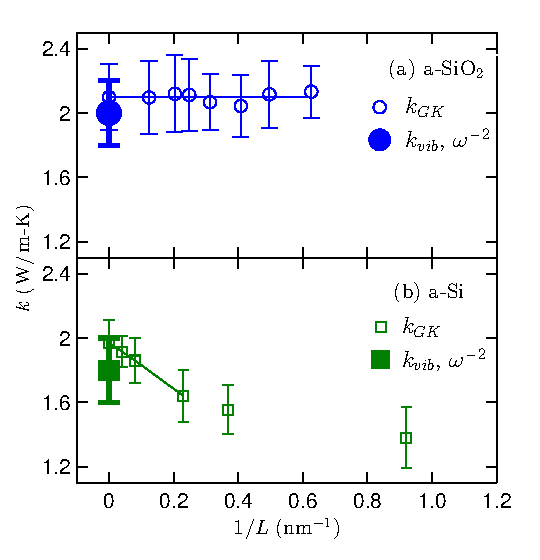
\includegraphics[scale=1.0]
{/home/jason/disorder/si/amor/m_af_si_normand_4096_gk_cond_4.eps}
\vspace*{-5mm}
\end{center}
\caption{\label{FIG:cond} Thermal conductivities of a-SiO$_2$ and 
a-Si predicted using the GK method and Eq. \eqref{EQ:kvib}. 
For a-SiO$_2$, the GK-predicted thermal conductivity 
is size-independent, indicating that there is no important 
contribution from propagating modes. For a-Si, there is a clear size 
dependance, indicating the importance of propagating modes. }
\end{figure}
%--------------------------------------------------------------------------
\clearpage
%--------------------------------------------------------------------------
\begin{center}
\begingroup
%\squeezetable
\begin{table}
\caption{\label{T:cond}
Total thermal conductivities for bulk a-SiO$_2$ and a-Si 
predicted by the GK method ($k_{GK}$) and 
Eq. \eqref{EQ:kvib} ($k_{vib}$). 
The total thermal conductivity $k_{vib}$ is predicted from the 
propagating [$k_{pr}$, Eq. \eqref{EQ:kph}] 
and non-propagating [$k_{pr}$, Eq. \eqref{EQ:kAF}] contributions. 
For the non-propagating contribution, classical and quantum 
specific heats are considered [Eq. \eqref{EQ:Cquantum}]. 
}
%\begin{ruledtabular}
\begin{tabular}{llllll}
\hline
Conductivity (W/m-K) & a-SiO$_2$ & a-Si & \\

\hline
$k_{GK}$ & 2.1 $\pm$ 0.2 & 2.0 $\pm$ 0.2 & \\
\hline
$k_{vib}$ & 2.0 $\pm$ 0.1 & 1.8 $\pm$ 0.2 & \\
\hline
$k_{pr}$ & 0.10 $\pm$ 0.05 & 0.6 $\pm$ 0.2 & \\
\hline
$k_{AF}$ (classical) & 1.9 $\pm$ 0.1 & 1.2 $\pm$ 0.1 & \\
\hline
$k_{AF}$ (quantum) & 1.4 $\pm$ 0.1 & 1.0 $\pm$ 0.1 & \\
\hline
$k_{vib}$ (quantum) & 1.5 $\pm$ 0.1 & 1.6 $\pm$ 0.2 & \\
\end{tabular}
%\end{ruledtabular}
\end{table}
\endgroup
\end{center}
%--------------------------------------------------------------------------
%\clearpage


% \begin{center}
% \begin{table}
% \begin{tabular}{llllll}
% \hline\hline
% $\phi$ & $L_{eq}$& $k$ (Matthiessen Rule w/$L_{eq}$)& $k$(Free Path Sampling)\\
% & (nm) & (W/m-K) & (W/m-K) \\
% \hline
% $0.1$ & $405$ & $91$ & $84$\\
% $0.2$ & $365$ & $89$ & $78$\\
% $0.3$ & $275$ & $85$ & $72$\\
% $0.4$ & $270$ & $85$ & $67$\\
% $0.5$ & $225$ & $82$ & $62$\\
% \hline\hline
% \end{tabular}
% \end{table}
% \end{center}

%--------------------------------------------------------------------------
\subsection{\label{S:Accumulation}Accumulation Function}
%--------------------------------------------------------------------------

The broadband frequency domain thermal-reflectance 
measurements by Regner et al.,\cite{regner_broadband_2013}  
following the suggestion of Koh and Cahill,\cite{koh_frequency_2007} 
interpret the  
measured thermal conductivity at a given penetration depth 
to be representative of the so-called thermal conductivity 
accumulation function.\cite{dames_thermal_2005,yang_mean_2013} 
Their results are plotted in Fig. \ref{FIG:sio2_accum} (a) 
for a 1000 nm thick film of a-SiO$_2$ 
and in Fig. \ref{FIG:sio2_accum} (b) for 500 nm and 
2000 nm thick films of a-Si. 
Based on the results in Section \ref{S:Diffusivities}, we will build 
thermal conductivity accumulation functions for a-SiO$_2$ and a-Si from
\begin{equation}\label{EQ:kLambda}
k(\Lambda_{max}) = k_{AF} + 
\frac{1}{V}\int^{\Lambda_{max}}_{\Lambda_{cut}} 
C(\Lambda) D(\Lambda)DOS(\Lambda)d\Lambda,
\end{equation}
where $\Lambda_{cut}$ is the MFP at the cut-off frequency, 
$\Lambda_{max}$ is the maximum MFP considered in the thermal 
conductivity accumulation, and the propagating mode MFPs are 
calculated using Eq. \eqref{EQ:Lambda}. The 
diffuson contribution $k_{AF}$ is evaluated using the quantum 
specific heat for a-SiO$_2$ (see Section \ref{S:Bulk}). 
The results are plotted 
in Figs. \ref{FIG:sio2_accum} (a) and \ref{FIG:sio2_accum} (b), 
alongside available experimental measurements on thin films. 
For a-Si, the experimental measurements are grouped 
broadly by sample preparation technique: 
(A) chemical vapor deposition
\cite{moon_thermal_2002,liu_high_2009,yang_anomalously_2010}
and 
(B) sputtered.
\cite{kuo_thermal_1992,cahill_thermal_1994,wada_thermal_1996} s

The predicted thermal conductivity accumulation function for a-SiO$_2$ 
saturates 
at a MFP of 10 nm, which is on the order of the finite size 
of our model.  
This result is in accord 
with the penetration depth-independent thermal 
conductivity measurements using broadband FDTR
\cite{regner_broadband_2013} and experimental measurements 
that show no film thickness dependance.
\cite{lee_heat_1997,yamane_measurement_2002} 
For a-Si, the low-MFP plateau of thermal conductivity in the   
measurements of Regner et al. is consistent with our 
predicted $k_{AF}$. 
The propagating contribution to the accumulation is predicted 
using both $\omega^{-2}$ and $\omega^{-4}$ scalings.  
As discussed in Section \ref{S:Conductivity}, 
the $\omega^{-2}$ scaling best describes the propagating 
contribution for our model of bulk a-Si. 
The thermal conductivity accumulation for the $\omega^{-2}$ 
scaling 
passes through the largest penetration 
depth measurements of Regner et al., as well as some of the  
experimental measurements for varying film thicknesses. 

We also consider the $\omega^{-4}$ scaling with the boundary 
scattering model [Eq. \eqref{EQ:LambdaMatth}] and an 80 $\mu$m 
thick film. 
The measurements of Regner et al. show much sharper accumulations 
than either the $\omega^{-2}$ or $\omega^{-4}$ scalings, 
particularly for a film of thickness $2$ $\mu$m. 
Because of the large variation in 
experimental measurements, predictions for both $\omega^{-2}$ 
and $\omega^{-4}$ pass reasonably well 
through the experimental measurements of Regner et al. and 
on thin films. 
Amorphous silicon is typically 
prepared as thin films,\cite{vacher_attenuation_1980} 
where voids and other inhomogeneities are unavoidable and can 
influence the vibrational structure at low frequencies.
\cite{feldman_tight-binding_2004,liu_high_2009,
yang_anomalously_2010,li_effect_2011,li_enhancement_2012} 
It is worth noting again 
that the results from thin film experiments have been interpreted 
using both $\omega^{-2}$ and $\omega^{-4}$ scalings.
\cite{feldman_thermal_1993,cahill_thermal_1994,
feldman_numerical_1999,liu_high_2009,yang_anomalously_2010} 

%--------------------------------------------------------------------------
% \begin{figure}
% \begin{center}
% \includegraphics[scale=1.0]
% {/home/jason/disorder/si/amor/m_af_si_normand_4096_kLamba_6_sio2.eps}
% \vspace*{-5mm}
% \end{center}
% \caption{\label{FIG:si_accum} Predicted thermal conductivity 
% accumulation function [Eq. \eqref{EQ:kLambda} 
% for a-SiO$_2$ compared with experimental measurements 
% by Regner et al.,\cite{regner_broadband_2013} 
% Love and Anderson (Expt. A),\cite{love_estimate_1990} 
% and Yamane et al. (Expt. B).\cite{yamane_measurement_2002}
% The predicted thermal conductivity accumulation demonstrates that 
% the propagating contribution is negligible in our model, which is 
% in accord with the experimental measurements.
% }
% \end{figure}
%--------------------------------------------------------------------------

%--------------------------------------------------------------------------
\begin{figure}
\begin{center}
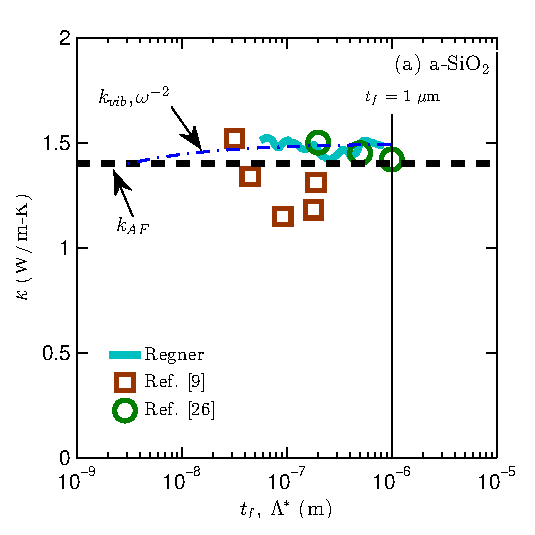
\includegraphics[scale=1.0]
{/home/jason/disorder/si/amor/m_af_si_normand_4096_kLamba_7_sio2_2.eps}
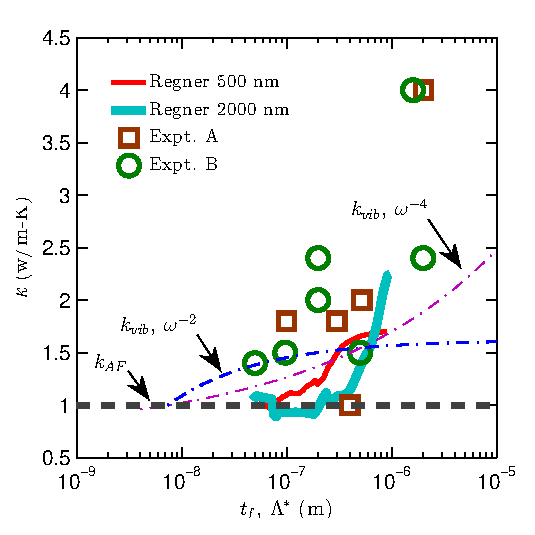
\includegraphics[scale=1.0]
{/home/jason/disorder/si/amor/m_af_si_normand_4096_kLamba_7_si.eps}
\vspace*{-5mm}
\end{center}
\caption{\label{FIG:sio2_accum} 
(a) predicted thermal conductivity 
accumulation function [Eq. \eqref{EQ:kLambda}]  
for a-SiO$_2$ compared with experimental measurements 
by Regner et al.,\cite{regner_broadband_2013} 
Yamane et al. (Expt. A),\cite{yamane_measurement_2002} and
Lee and Cahill (Expt. B).\cite{lee_heat_1997} 
The predicted thermal conductivity accumulation demonstrates that 
the propagating contribution is negligible in our model, which is 
in accord with the experimental measurements. 
(b) predicted thermal conductivity 
accumulation function 
for a-Si compared with experimental measurements 
by Regner et al. and of 
sputtered (Expt. A),
\cite{kuo_thermal_1992,wada_thermal_1996,cahill_thermal_1994} 
and chemical vapor deposited (Expt. B)
\cite{hasselman_thermal_1989,moon_thermal_2002,liu_high_2009,
yang_anomalously_2010} 
thin films with a wide-range of film thicknesses. 
The predicted thermal conductivity accumulation demonstrates that 
the propagating contribution is significant for a-Si, while the 
agreement with the various experimental measurements is only 
qualitatively. 
}
\end{figure}
%--------------------------------------------------------------------------
\clearpage

%\vspace{50mm}

%%--------------------------------------------------------------------------
%\subsection{\label{S:Discussion}Discussion}
%%--------------------------------------------------------------------------

% The transverse sound speed predicted for our model of 
% a-SiO$_2$ is about $85\%$ of that predicted by 
% the other methods used in the present study and that 
% measured by experiment.\cite{liu_high_2009}  
% While using a smaller transverse sound speed 
% leads to an underprediction of the 
% mode diffusivity scalings (Eq. \eqref{EQ:Dtau},
% Fig. \ref{FIG:diffusivities} ), it leads to an 
% overprediction of the DOS (Eq. \eqref{EQ:DOS_debye}). 
% Holding all other input parameters in Eq. \eqref{EQ:kvib} constant, 
% a smaller sound speed leads to a larger $k_{pr}$ 
% prediction because the DOS scales as 
% $DOS(\omega)\propto 1/v^3_{s}$. In this sense we can regard 
% the prediction for $k_{pr}$ from 
% our model of a-SiO$_2$ with reduced transverse sound speeds  
% as an upper bound. 
% Our model confirms that propagating modes do not contribute significantly 
% to the thermal conductivity of a-SiO$_2$.

% While experiments show there is a cross-over region for the 
% low-frequency diffusivity scaling from $n=2$ to $n=4$ scaling,
% \cite{masciovecchio_evidence_2006,baldi_emergence_2013} 
% the propagating contribution was still negligible. 
% The cross-over region from $n=2$ to $n=4$ observed in experiments for  
% a-SiO$_2$ occurs in the frequency range $4.6 10^9$ to 
% $1.52 10^{10}$ rads$/$s,\cite{masciovecchio_evidence_2006} 
% and $3.04 10^11$ to $1.52 10^{12}$ rads$/$s
% \cite{baldi_emergence_2013}. 
% Our present model is not 
% large enough to investigate the cross-over region for $n=2$ to 
% $n=4$ scaling. The required model size will most likely 
% keep the required frequency range inaccessible for some 
% time to come. 

% A transition between $n=2$ and $n=4$ scaling can be 
% achieved using a phenomenological model where a cross-over frequency 
% must be specified by experiment.
% \cite{baldi_elastic_2011} While this cross-over can be identified 
% experimentally for a-SiO$_2$,\cite{masciovecchio_evidence_2006} 
% experiments are limited for a-Si thin films.(cite) 
% Our model for bulk a-Si seems best described by a propagating 
% contribution $k_{pr}$ using Eq. \eqref{EQ:Dw2} with $n=2$ (see Fig. ). 
% Using the boundary 
% scattering model Eq. \eqref{matth} to  predict the thermal conductivity 
% accumulation function in Fig. with $n=2$ and $n=4$ shows that 
% the experimental measurements for a-Si thin films are still not 
% well-understood. Our model can describe the accumulations predicted 
% by broadband FDTR measurements by Regner only qualitatively in the 
% short and long MFP limits. 
% While the low-frequency scaling of the 
% diffusivities has been investigated experimentally for a-SiO$_2$, 
% experimental measurements for a-Si are lacking. Measurements 
% of the thermal conductivity of a-Si thin films with varying 
% temperature suggest both 
% $n=2$(cite) and 
% $n=4$(cite) 
% separately based on varying preparation techniques. 

% This supports the idea of Slack for a-SiO$_2$\cite{slack_thermal_1979}
% While the thermal conductivity of a-SiO , the material is characterized by 
% a constant similar for other amorphous
% materials such as Lennard-Jones argon\cite{larkin_predicting_2013} 
% and a model of a-GeTe.\cite{sosso_thermal_2012}
% 
% That the amorphous phase
% of Si should have a lower GHz attenuation than many other
% amorphous materials is not entirely surprising, as the 2002
% review of low-temperature thermal conductivity and internal
% friction by Pohl, Liu, and Thompson certainly indicates that
% the fourfold coordinated materials tend to demonstrate weaker
% anharmonicity.\cite{pohl_low-temperature_2002}
% 
% Theoretical predictions of acoustic attenuation in amor-
% phous solids generally agree that at room temperature, a
% quadratic frequency dependence is expected in the frequency
% range of 10 GHz–1 THz and its origins are expected to be
% the anharmonicity of the interatomic bonds.
% 
% Theory from Schirmacher et al. predicted 
% an w4 scaling below a system dependent onset frequency.
% \cite{schirmacher_thermal_2006,schirmacher_acoustic_2007}

%--------------------------------------------------------------------------
\section{\label{S:Lifetimes}Summary}
%--------------------------------------------------------------------------

In this work we investigated the contributions of propagating ($k_{ph}$) 
and non-propagating ($k_{AF}$) modes to the total vibrational 
thermal conductivity $k_{vib}$ of two amorphous materials, 
a-SiO$_2$ and a-Si, using the GK method (Section \ref{S:Bulk}), 
NMD method (Section \ref{S:Life}),  
and AF theory (Section \ref{S:Diffusivities}). 
For our model of bulk a-Si, 
the thermal conductivity has  
significant contribution from propagating modes which are best 
described by a diffusivity scaling of $\omega^{-2}$ 
(see Section \ref{S:Theory:Thermal}).  
For a-SiO$_2$, the contribution from propagating modes was shown to 
be negligible (Section \ref{S:Bulk}). 
The is confirmed by experimental thin film measurements
\cite{love_estimate_1990,baldi_thermal_2008} 
and broadband frequency domain thermal reflectance measurements  
by Regner et al.\cite{regner_broadband_2013} 

The thermal conductivity accumulation functions predicted for a-Si 
using both $\omega^{-2}$ 
and $\omega^{-4}$ scalings show reasonable agreement 
with the experimental measurements from Regner et al.
\cite{regner_broadband_2013} and on thin films.
\cite{feldman_thermal_1993,cahill_thermal_1994,
feldman_numerical_1999,liu_high_2009,yang_anomalously_2010} 
In fact, the existence of $\omega^{-2}$ and/or $\omega^{-4}$ 
scalings has been argued on the basis of the low-temperature 
($< 10$ K)
thermal conductivity plateau,
\cite{freeman_thermal_1986,feldman_thermal_1993,
feldman_numerical_1999} 
which is observable in some preparations of a-SiO$_2$
\cite{zeller_thermal_1971,freeman_thermal_1986,
cahill_lattice_1988,cahill_heat_1989} 
and a-Si\cite{pompe_thermal_1988,liu_high_2009}, 
but absent in others.
\cite{zink_excess_2006,zink_thermal_2006,liu_high_2009} 

The large discrepancies between measurements of 
a-Si thin films suggest that a comprehensive 
experimental study using the recently developed broadband 
techniques\cite{koh_frequency_2007,
minnich_thermal_2011,regner_broadband_2013} on varying film 
thicknesses and preparation techniques is necessary.  
It may be particularly helpful to perform the experiments 
at temperatures less than $< 10$ K where the propagating contribution 
dominates for both a-SiO$_2$ and a-Si and the low-frequency scaling 
is still up for debate.\cite{freeman_thermal_1986,
cahill_lattice_1988,cahill_thermal_1989,
love_estimate_1990,feldman_thermal_1993,cahill_thermal_1994,
feldman_numerical_1999,baldi_thermal_2008,liu_high_2009,
yang_anomalously_2010} 
Recent thermal conductivity measurements at room temperature 
of suspended amorphous silicon nitride bridges showed significant 
contributions from long MFP 
vibrations to heat transport,\cite{sultan_heat_2013} 
which provides a comparison material to a-Si that deserves further 
investigation. 

\begin{acknowledgements}
This work was supported by AFOSR award FA95501010098 and by a grant 
of computer time from the DOD 
High Performance Computing Modernization Program at the US Army 
Engineer 
Research and Development Center. 
We thank Davide Donadio, Joseph Feldman, Asad Hasan, Jonathan Malen,  
Craig Maloney, Normand Mousseau, Keith Regner, and Michael Widom 
for helpful discussions.
\end{acknowledgements}

%\clearpage
\bibliographystyle{apsrev}
\bibliography{/home/jason/Dropbox/ntpl-paper/ntpl-072613}
\end{document}
% 